\chapter{Background}\label{sec:chapter2}

In this chapter the mathematical background that later chapters rely on is introduced.
\cref{sec:chapter2_signals_sphere} begins with a review of signals on the sphere on which much of this work is built.
Localised spatial-scale analysis is considered through wavelets in \cref{sec:chapter2_wavelets}, followed by localised spatial-spectral analysis via the Slepian concentration problem in \cref{sec:chapter2_slepian_concentration_problem}.
The primary motivation behind this work, namely: observations over the partial sphere in cosmology is discussed in \cref{sec:chapter2_motivation}.
Lastly, limitations of existing approaches and the aim of this thesis is covered in \cref{sec:chapter2_outlook}.

\section{Signals on the Sphere}\label{sec:chapter2_signals_sphere}

Much of this thesis is based on signals on the sphere, and as such some appropriate mathematical background is introduced here.
Signals on the sphere arise in many areas of science and engineering, including: cosmology~\cite{Bennett1996}, geophysics~\cite{Simons2006}, planetary science~\cite{Turcotte1981}, quantum chemistry~\cite{Choi1999}, computer vision~\cite{Cohen2018,Esteves2020,Cobb2021}, and computer graphics~\cite{Ramamoorthi2004}.

\subsection{Notation}

The 2-sphere \(\twoSphere{}\) is defined as
%
\begin{equation}
	\twoSphere{}
	%
	= \set{\omega \in \mathbb{R}^{3} : \norm{\omega} = 1},
\end{equation}
%
where \(\omega=(\theta,\phi)\) parameterise a point on the unit sphere, \(\theta \in \interval{0}{\pi}\) is the colatitude and \(\phi \in \interval[open right]{0}{2\pi}\) is the longitude.
The Hilbert space \(\hilbert{\twoSphere}\) is formed by the complex valued square-integrable functions \(\pixel{f}\), \(\pixel{g}\), with inner product
%
\begin{equation}
	\braket*{f}{g}
	%
	= \integrateSphere{\omega} \pixel{f} \pixel{\conj{g}},
\end{equation}
%
where \(\sphereVolume{} = \sin{\theta} \dd{\theta} \dd{\phi}\) is the usual rotation invariant measure on the sphere.
The complex inner product induces a norm
%
\begin{equation}
	\norm{f}
	%
	= \sqrt{\braket*{f}}.
\end{equation}
%
Signals on the sphere are functions with a finite induced norm.

\subsection{Spherical Harmonics}

The spherical harmonics \(\pixel{\harmonic{Y}}\), with integer degree \(\ell \geq 0\) and integer order \(m \leq \abs{\ell}\), form an orthonormal basis of the Hilbert space \(\hilbert{\twoSphere}\).
Consider the Laplacian in spherical coordinates
%
\begin{equation}
	\laplacian
	%
	= \frac{1}{r^{2}} \pdv{r} \bigg(r^{2} \pdv{r}\bigg)
	%
	+ \frac{1}{r^{2}\sin{\theta}} \pdv{\theta} \bigg(\sin{\theta} \pdv{\theta}\bigg)
	%
	+ \frac{1}{r^{2}\sin^{2}{\theta}} \pdv[2]{\phi}.
\end{equation}
%
The spherical harmonics are found by solving the Laplace equation
%
\begin{equation}\label{eq:chapter2_laplace}
	\laplacian{f(r,\theta,\phi)}
	%
	= 0,
\end{equation}
%
and substituting in a separation of variables
%
\begin{equation}
	f(r,\theta,\phi)
	%
	= R(r)\Theta(\theta)\Phi(\phi).
\end{equation}
%
Inserting this decomposition into the Laplace equation \cref{eq:chapter2_laplace}, and multiplying by \(r^{2}\sin^{2}{\theta}/R\Theta\Phi{}\) yields
%
\begin{equation}\label{eq:chapter2_laplace_m2}
	\frac{1}{\Phi} \pdv[2]{\Phi}{\phi}
	%
	= -\frac{\sin^{2}{\theta}}{R} \dv{r} \bigg(r^{2} \dv{R}{r}\bigg)
	%
	- \frac{\sin{\theta}}{\Theta} \dv{\theta} \bigg(\sin{\theta} \dv{\Theta}{\theta}\bigg)
	%
	= -m^{2},
\end{equation}
%
where \(-m^{2}\) is a constant chosen such that the solutions for \(\Phi(\phi)\) are periodic in \(\phi{}\), \ie{}
%
\begin{equation}
	\Phi(\phi)
	%
	= \exp(\pm i m\phi).
\end{equation}
%
Now, after dividing through by \(\sin^{2}{\theta}\), \cref{eq:chapter2_laplace_m2} may be recast as
%
\begin{equation}
	\frac{1}{R} \dv{r} \bigg(r^{2} \dv{R}{r}\bigg)
	%
	= -\frac{1}{\Theta\sin{\theta}} \dv{\theta} \bigg(\sin{\theta} \dv{\Theta}{\theta}\bigg)
	%
	+ \frac{m^{2}}{\sin^{2}{\theta}}
	%
	= \ell(\ell+1),
\end{equation}
%
where \(\ell(\ell+1)\) is a constant, the choice of which will become clear.
Through a change of variables \(x=\cos{\theta}\) and \(y=\Theta(\theta)\), the polar angle part reduces to
%
\begin{equation}
	(1-x^{2}) \dv[2]{y}{x} - 2x\dv{y}{x} + \bigg[\ell(\ell+1) - \frac{m^{2}}{(1 - x^{2})}\bigg] y
	%
	= 0,
\end{equation}
%
which is the differential equation for the associated Legendre polynomials \(y(x) = P^{m}_{\ell}(x)\).
The spherical harmonics are then formed by combining the solutions in the polar angle \(\theta{}\) and azimuthal angle \(\phi{}\) with a suitable normalisation factor by
%
\begin{equation}
	\pixel{\harmonic{Y}}
	%
	= \phaseFactor \sqrt{\factor \frac{(\ell-m)!}{(\ell+m)!}} P^{m}_{\ell}(\cos{\theta}) \exp(i m\phi).
\end{equation}
%
Included here is the Condon-Shortley \(\phaseFactor{}\) phase factor, to ensure the following conjugate symmetry relation holds
%
\begin{equation}
	\pixel{\conj{\harmonic{Y}}}
	%
	= \phaseFactor \pixel{Y_{\ell(-m)}}.
\end{equation}
%
The spherical harmonics satisfy the below orthonormality and completeness relations by
%
\begin{equation}\label{eq:chapter2_spherical_harmonics_orthonormal}
	\integrateSphere{\omega} \pixel{\harmonic{Y}} \pixel{\conj{\harmonic[']{Y}}}
	%
	= \delta_{\ell\ell'} \delta_{mm'},
\end{equation}
%
and
%
\begin{equation}
	\sum\limits_{\ell=0}^{\infty} \sum\limits_{m=-\ell}^{\ell} \pixel{\harmonic{Y}} \pixel[']{\conj{\harmonic{Y}}}
	%
	= \delta(\omega-\omega')
\end{equation}
%
respectively, where
%
\begin{equation}
	\delta(\omega-\omega')
	%
	= \delta(\phi-\phi') \delta(\cos{\theta} - \cos{\theta'})
\end{equation}
%
and \(\delta(x),\ x \in \mathbb{R}\) is the Dirac delta function.
A function on the sphere \(f \in \hilbert{\twoSphere}\) may be decomposed into this basis by
%
\begin{equation}
	\pixel{f}
	%
	= \sum\limits_{\ell=0}^{\infty} \sum\limits_{m=-\ell}^{\ell} \harmonic{f} \pixel{\harmonic{Y}},
\end{equation}
%
where \(\harmonic{f}\) are the spherical harmonic coefficients given by
%
\begin{equation}
	\harmonic{f}
	%
	= \integrateSphere{\omega} \pixel{f} \pixel{\conj{\harmonic{Y}}}.
\end{equation}
%
The conjugate symmetry relation of the spherical harmonic coefficients of a real function is
%
\begin{equation}
	\conj{\harmonic{f}}
	%
	= \phaseFactor f_{\ell(-m)}.
\end{equation}
%
A useful relation for the spherical harmonics is the addition theorem which states
%
\begin{equation}\label{eq:chapter2_addition_theorem}
	\sum\limits_{m=-\ell}^{\ell} \pixel{\harmonic{Y}} \pixel[']{\conj{\harmonic{Y}}}
	%
	= \factor P_{\ell}(\omega \cdot \omega'),
\end{equation}
%
where \(P_{\ell}(x)\) are the Legendre polynomials.
A pictorial representation of the spherical harmonics is given in \cref{fig:chapter2_spherical_harmonics}.

\begin{figure}[htpb]
	\capstart{}
	\subfloat[\(\pixel{Y_{00}}\)]
	{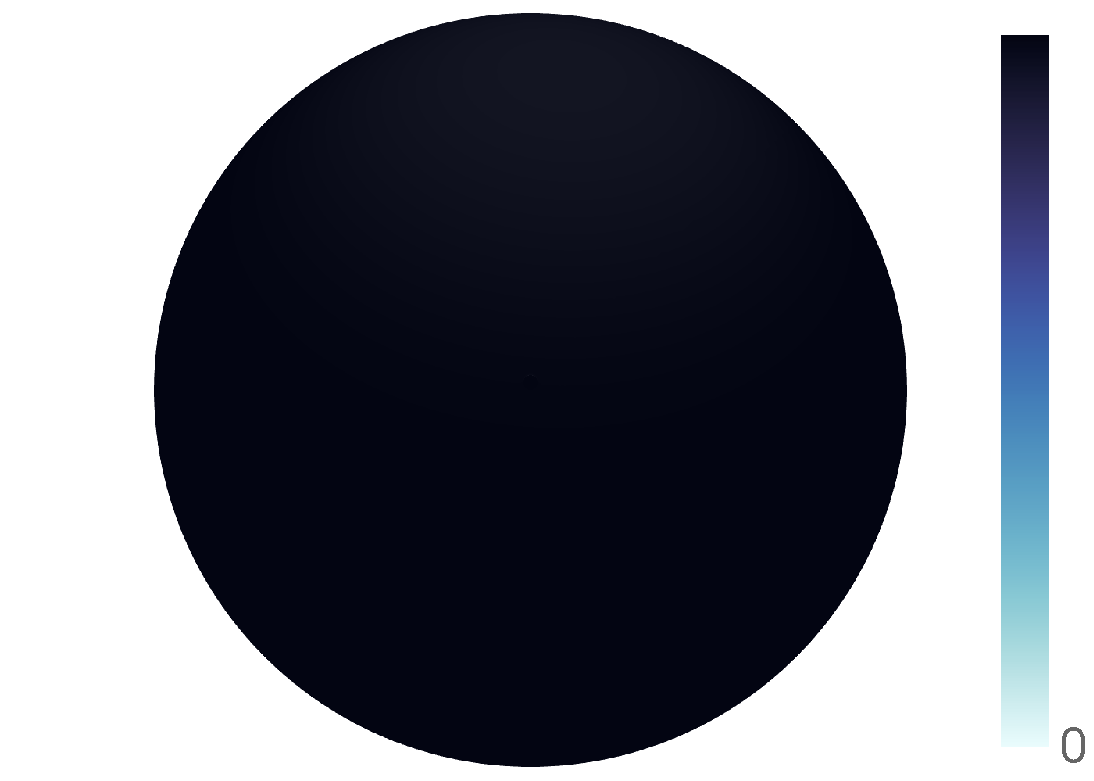
\includegraphics[trim={23 7 3 6},clip,width=.2\textwidth]{spherical_harmonic_0l_0m_L128_real_norm.pdf}}
	\newline
	\subfloat[\(\pixel{Y_{10}}\)]
	{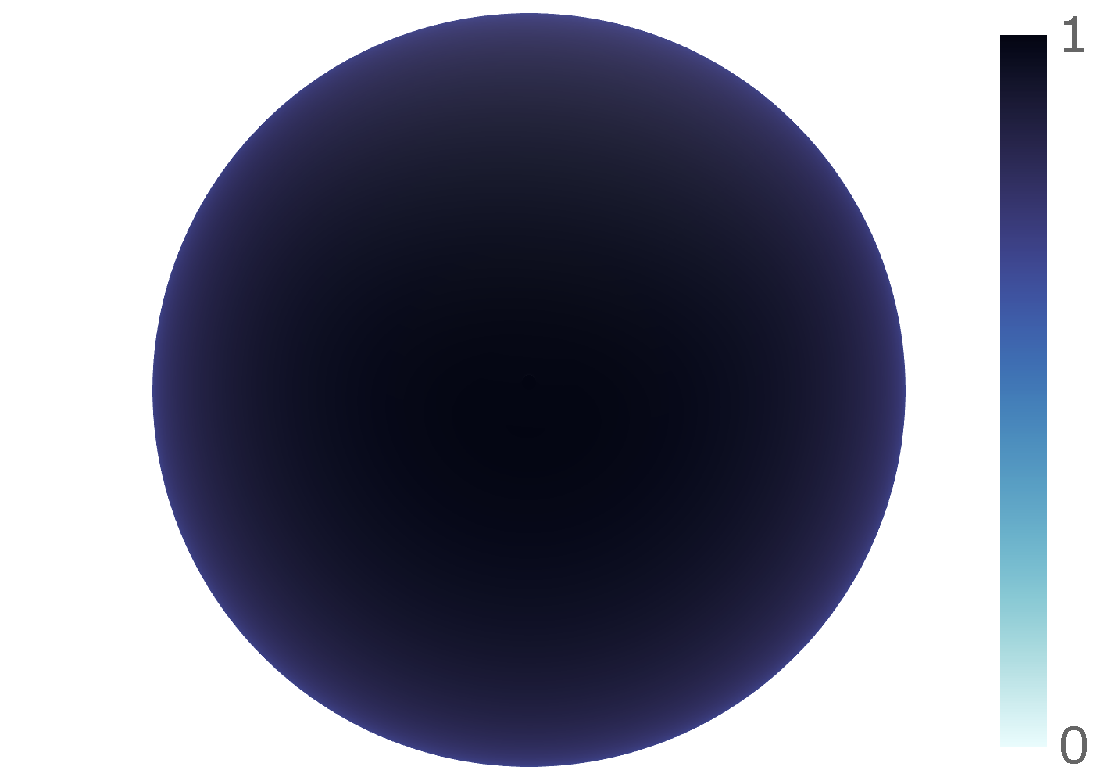
\includegraphics[trim={23 7 3 6},clip,width=.2\textwidth]{spherical_harmonic_1l_0m_L128_real_norm.pdf}}
	%
	\subfloat[\(\pixel{Y_{11}}\)]
	{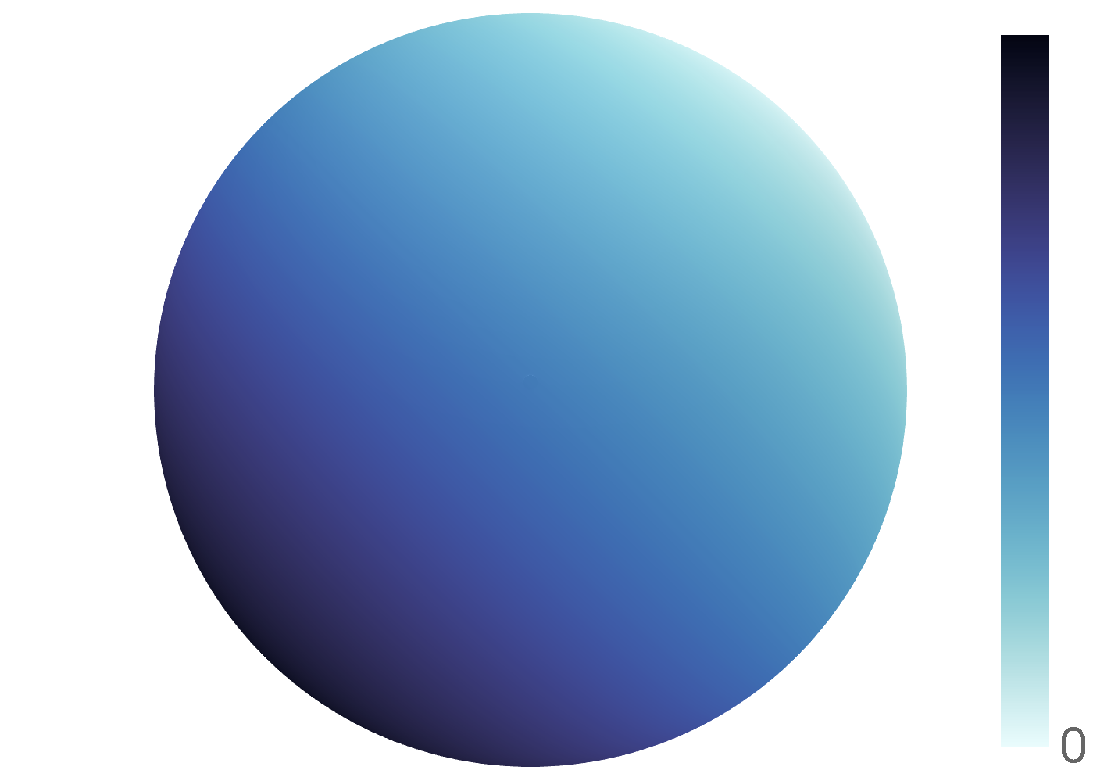
\includegraphics[trim={23 7 3 6},clip,width=.2\textwidth]{spherical_harmonic_1l_1m_L128_real_norm.pdf}}
	\newline
	\subfloat[\(\pixel{Y_{20}}\)]
	{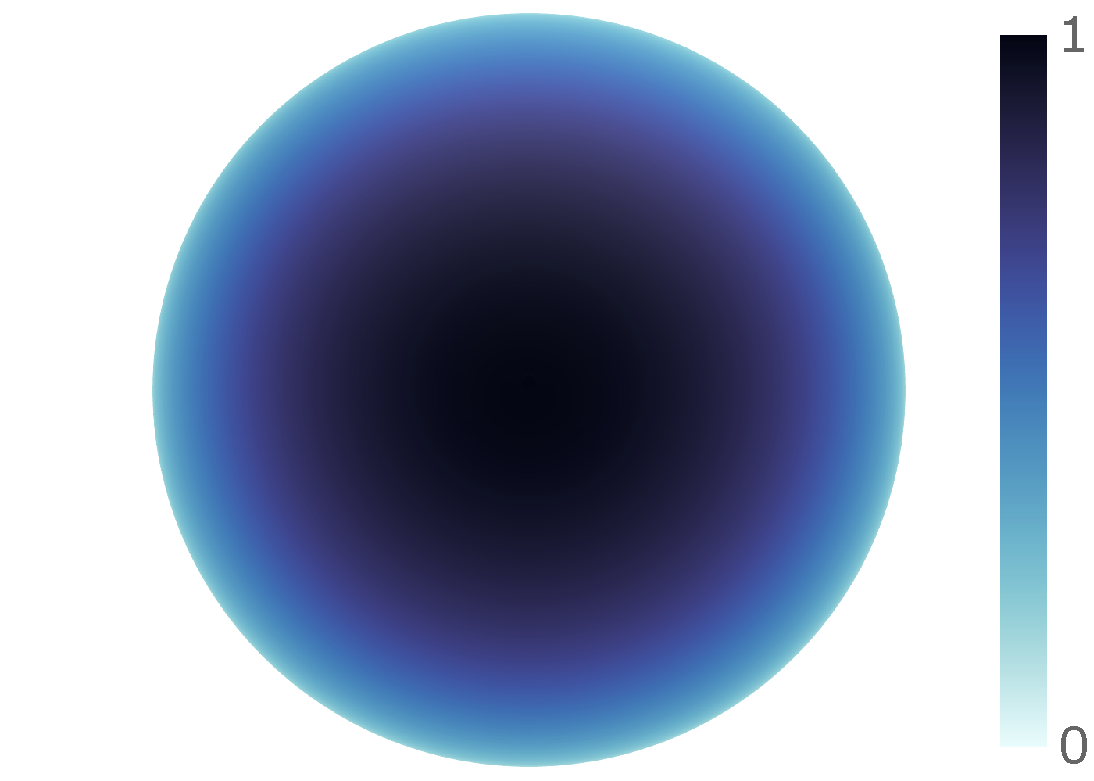
\includegraphics[trim={23 7 3 6},clip,width=.2\textwidth]{spherical_harmonic_2l_0m_L128_real_norm.pdf}}
	%
	\subfloat[\(\pixel{Y_{21}}\)]
	{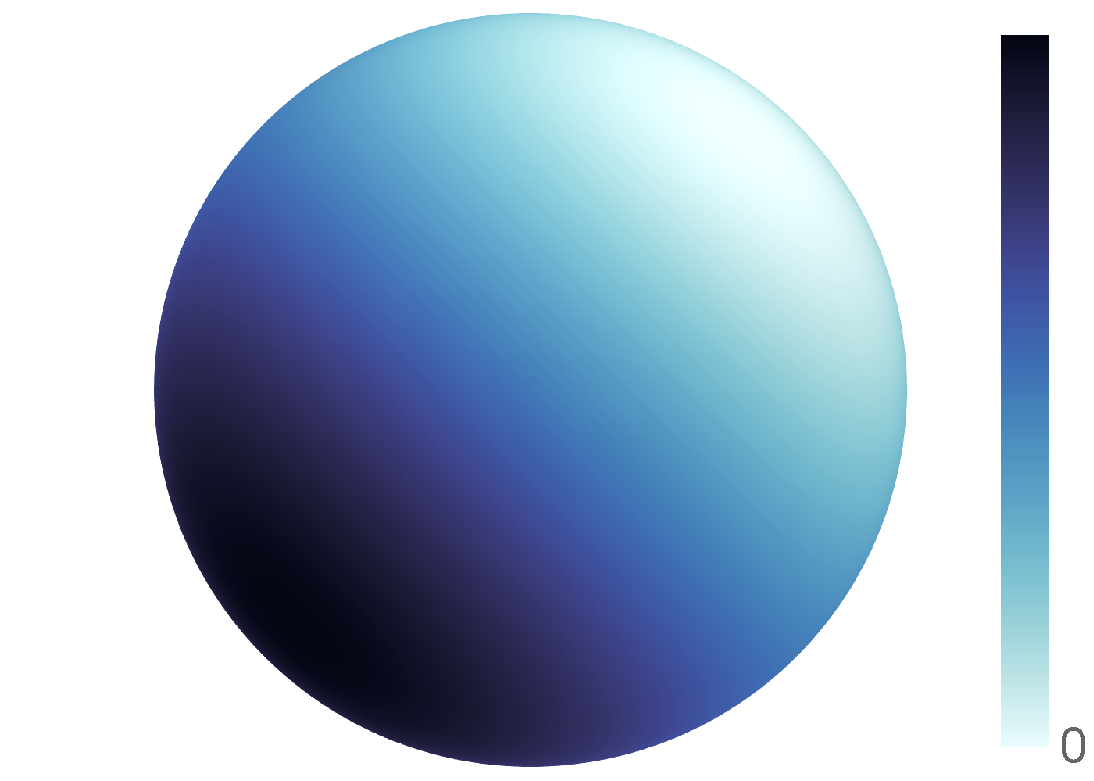
\includegraphics[trim={23 7 3 6},clip,width=.2\textwidth]{spherical_harmonic_2l_1m_L128_real_norm.pdf}}
	%
	\subfloat[\(\pixel{Y_{22}}\)]
	{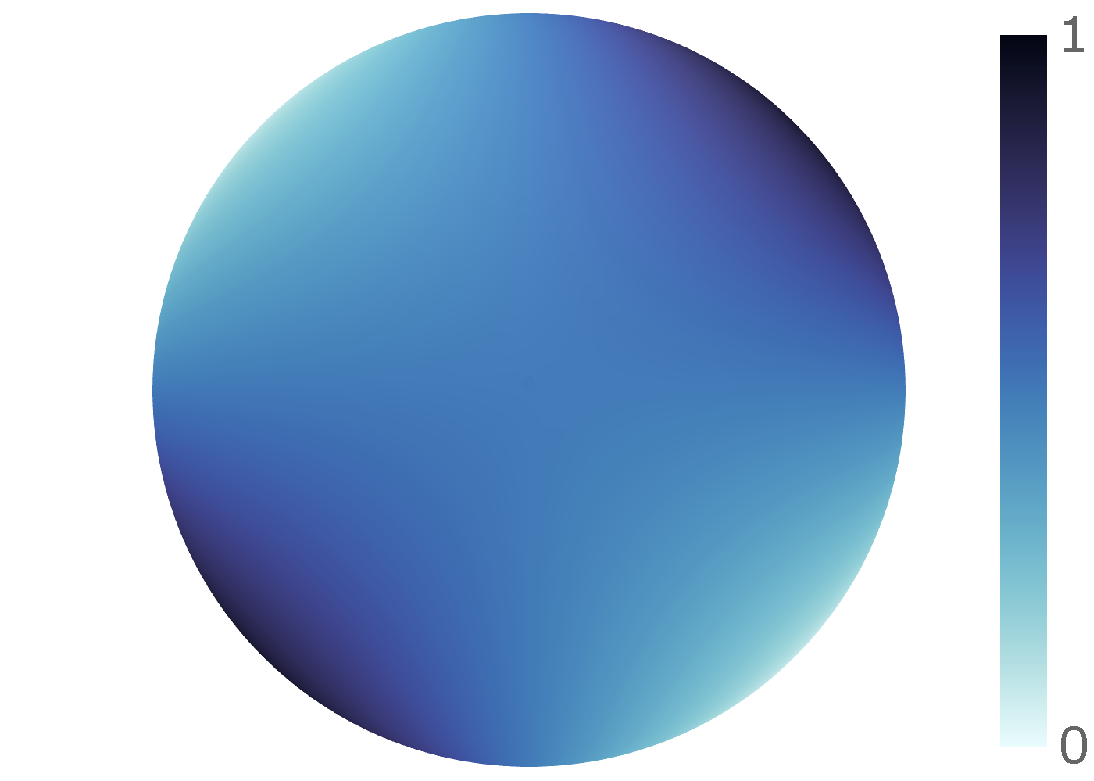
\includegraphics[trim={23 7 3 6},clip,width=.2\textwidth]{spherical_harmonic_2l_2m_L128_real_norm.pdf}}
	\newline
	\subfloat[\(\pixel{Y_{30}}\)]
	{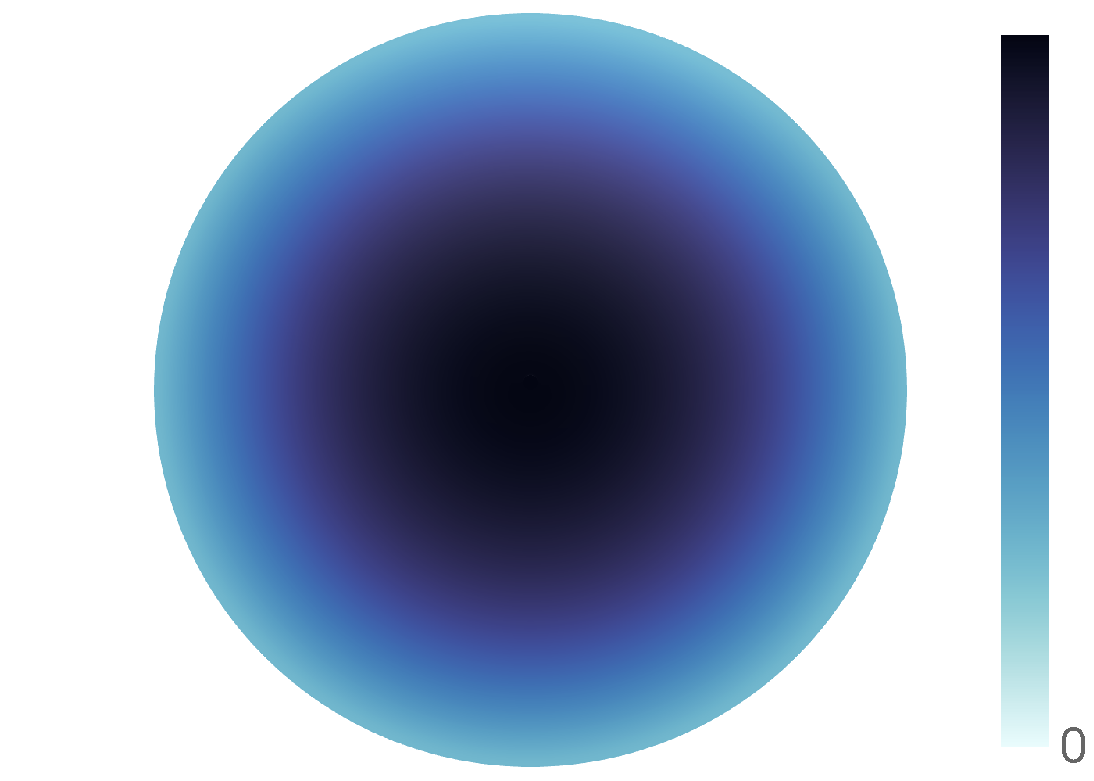
\includegraphics[trim={23 7 3 6},clip,width=.2\textwidth]{spherical_harmonic_3l_0m_L128_real_norm.pdf}}
	%
	\subfloat[\(\pixel{Y_{31}}\)]
	{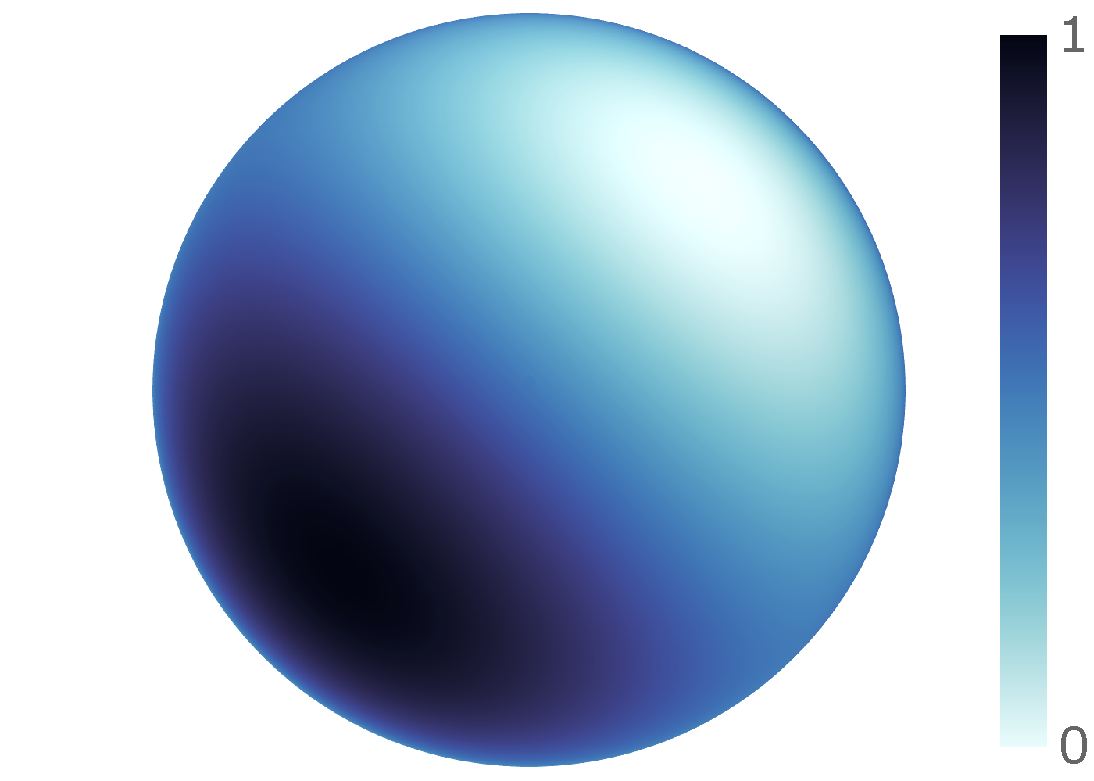
\includegraphics[trim={23 7 3 6},clip,width=.2\textwidth]{spherical_harmonic_3l_1m_L128_real_norm.pdf}}
	%
	\subfloat[\(\pixel{Y_{32}}\)]
	{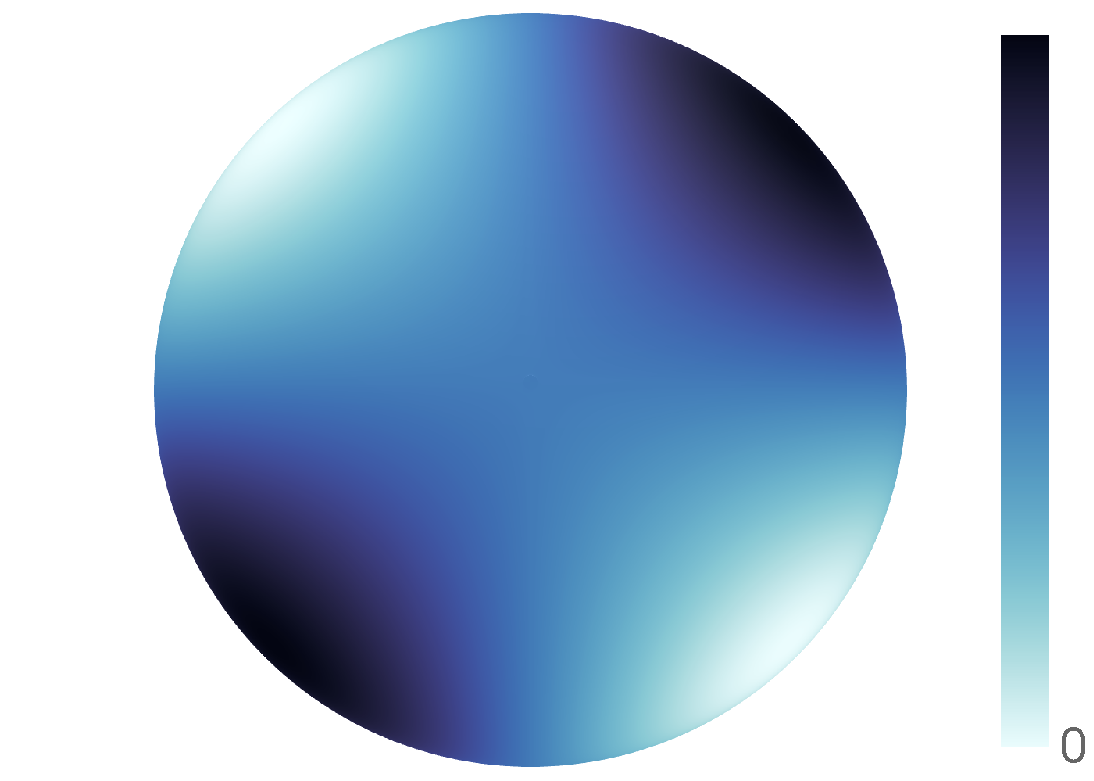
\includegraphics[trim={23 7 3 6},clip,width=.2\textwidth]{spherical_harmonic_3l_2m_L128_real_norm.pdf}}
	%
	\subfloat[\(\pixel{Y_{33}}\)]
	{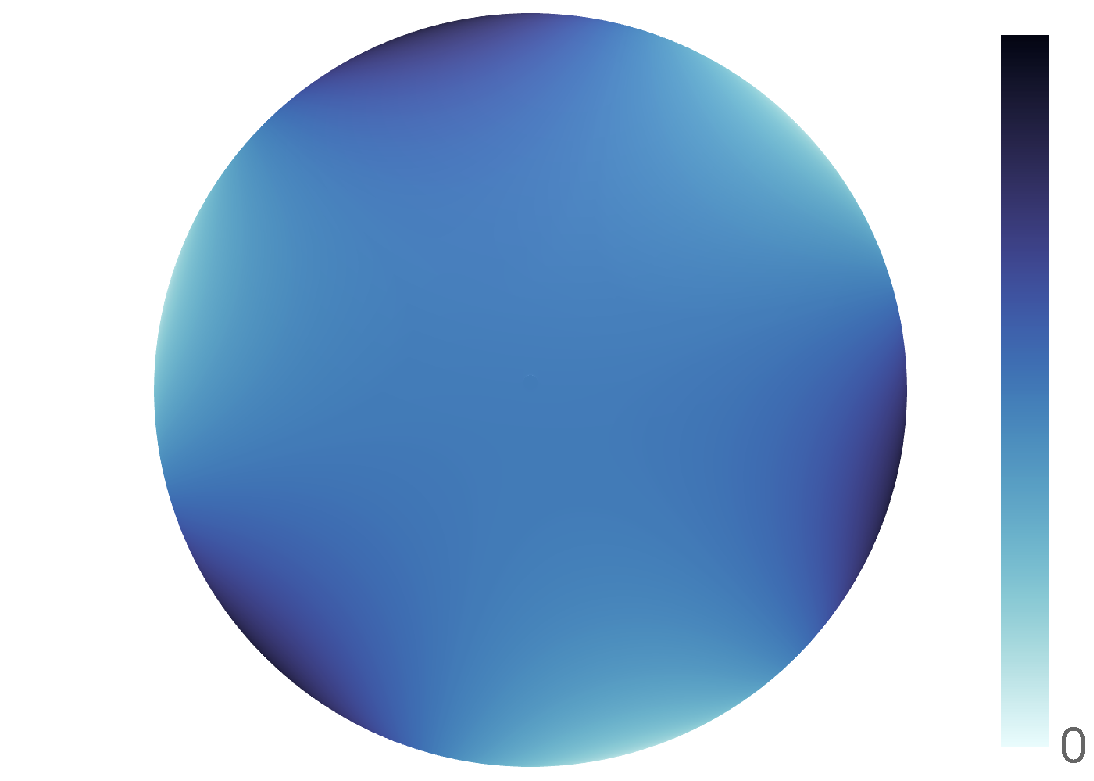
\includegraphics[trim={23 7 3 6},clip,width=.2\textwidth]{spherical_harmonic_3l_3m_L128_real_norm.pdf}}
	\newline
	\subfloat[\(\pixel{Y_{40}}\)]
	{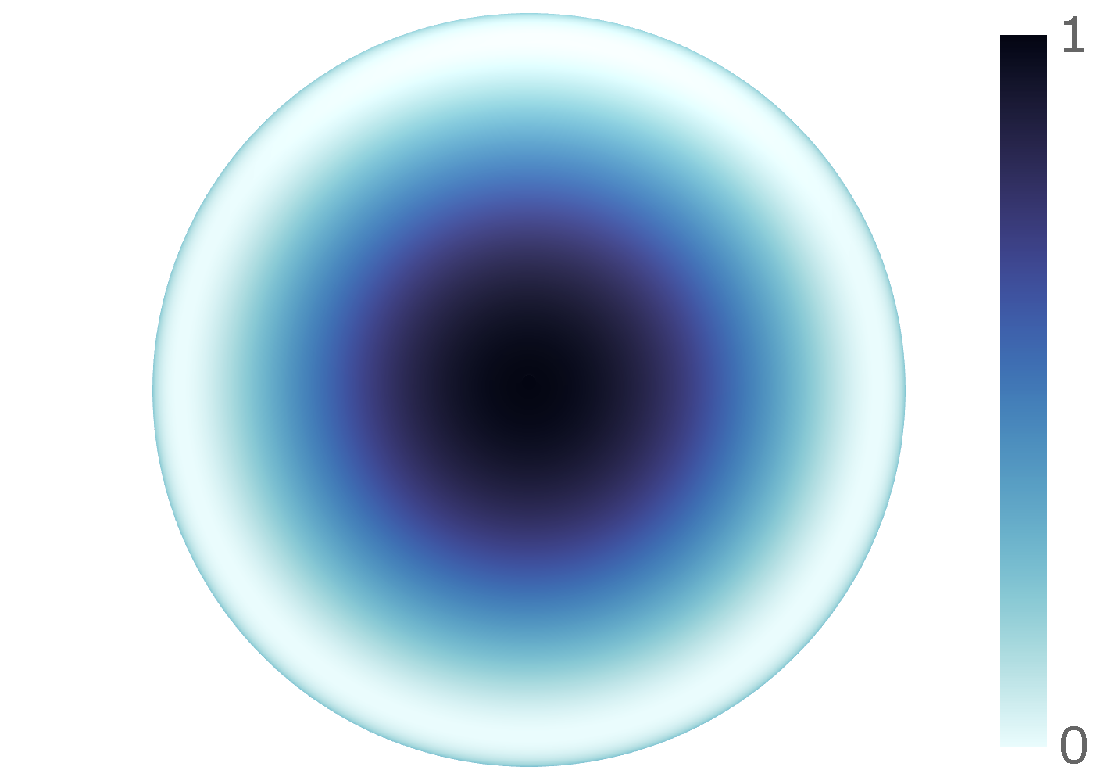
\includegraphics[trim={23 7 3 6},clip,width=.2\textwidth]{spherical_harmonic_4l_0m_L128_real_norm.pdf}}
	%
	\subfloat[\(\pixel{Y_{41}}\)]
	{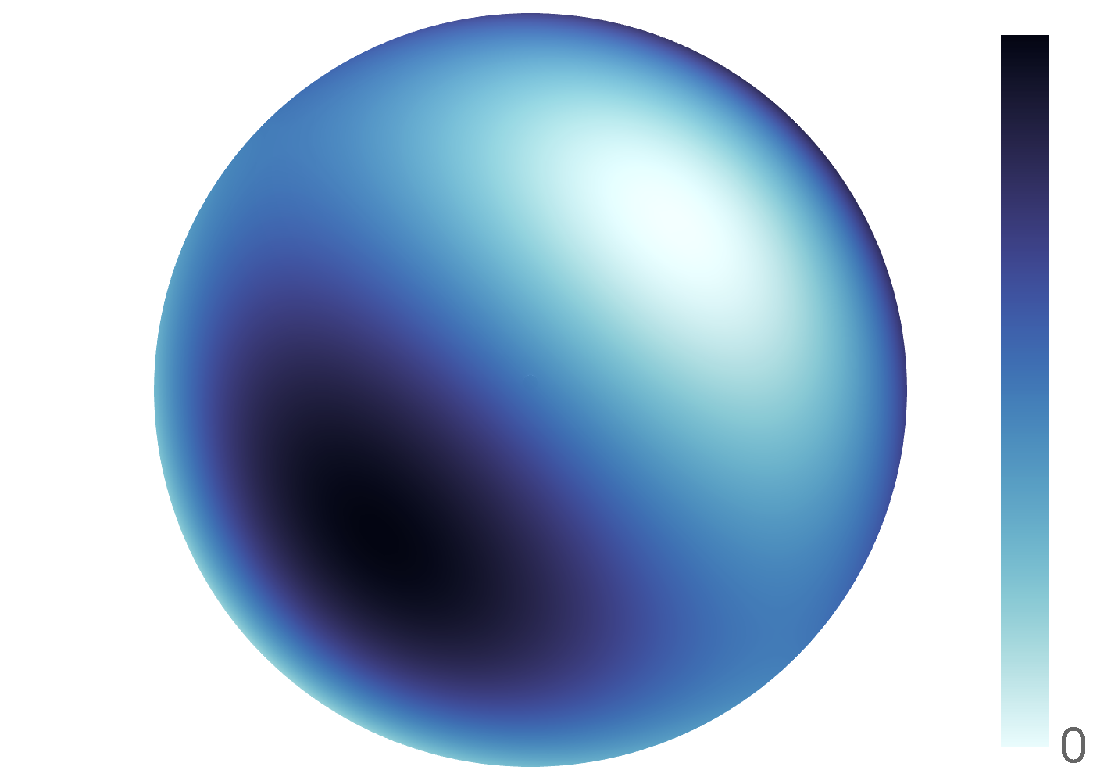
\includegraphics[trim={23 7 3 6},clip,width=.2\textwidth]{spherical_harmonic_4l_1m_L128_real_norm.pdf}}
	%
	\subfloat[\(\pixel{Y_{42}}\)]
	{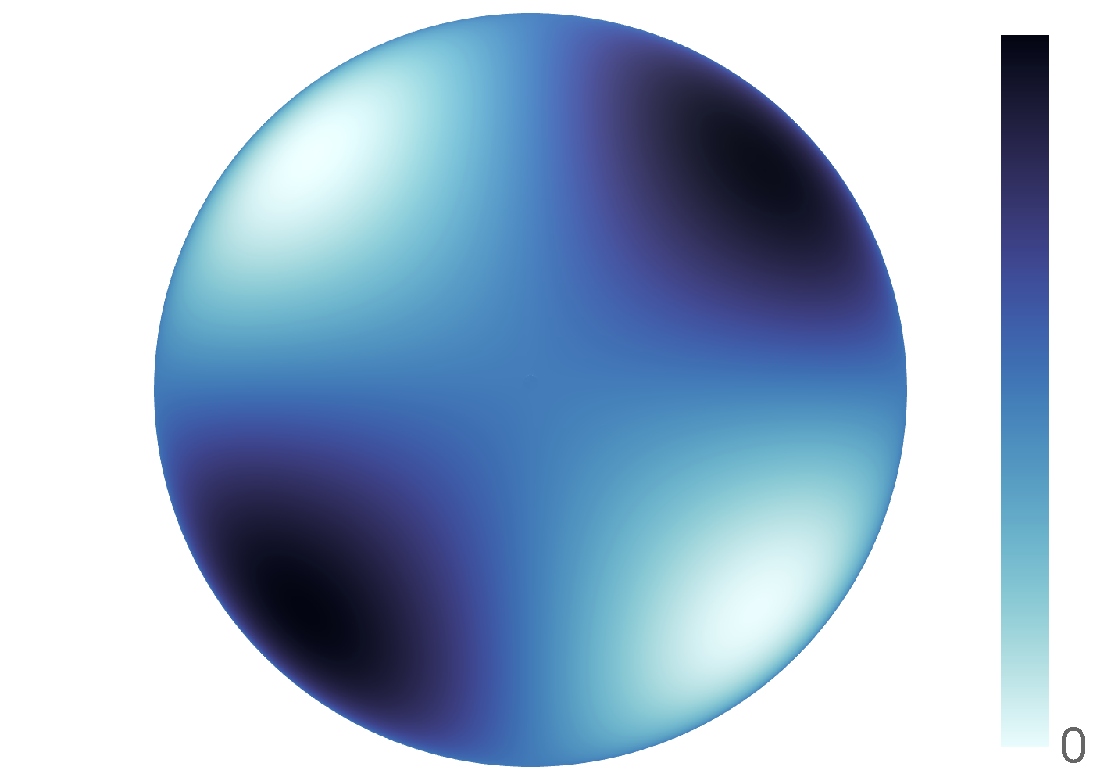
\includegraphics[trim={23 7 3 6},clip,width=.2\textwidth]{spherical_harmonic_4l_2m_L128_real_norm.pdf}}
	%
	\subfloat[\(\pixel{Y_{43}}\)]
	{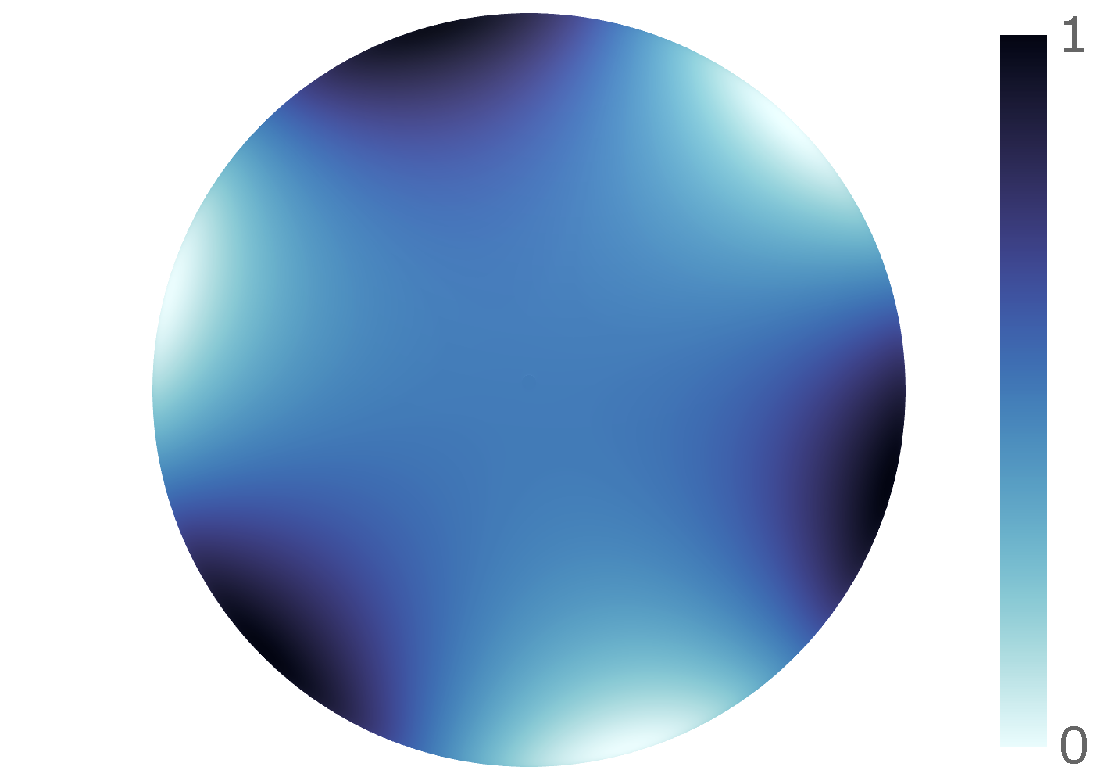
\includegraphics[trim={23 7 3 6},clip,width=.2\textwidth]{spherical_harmonic_4l_3m_L128_real_norm.pdf}}
	%
	\subfloat[\(\pixel{Y_{44}}\)]
	{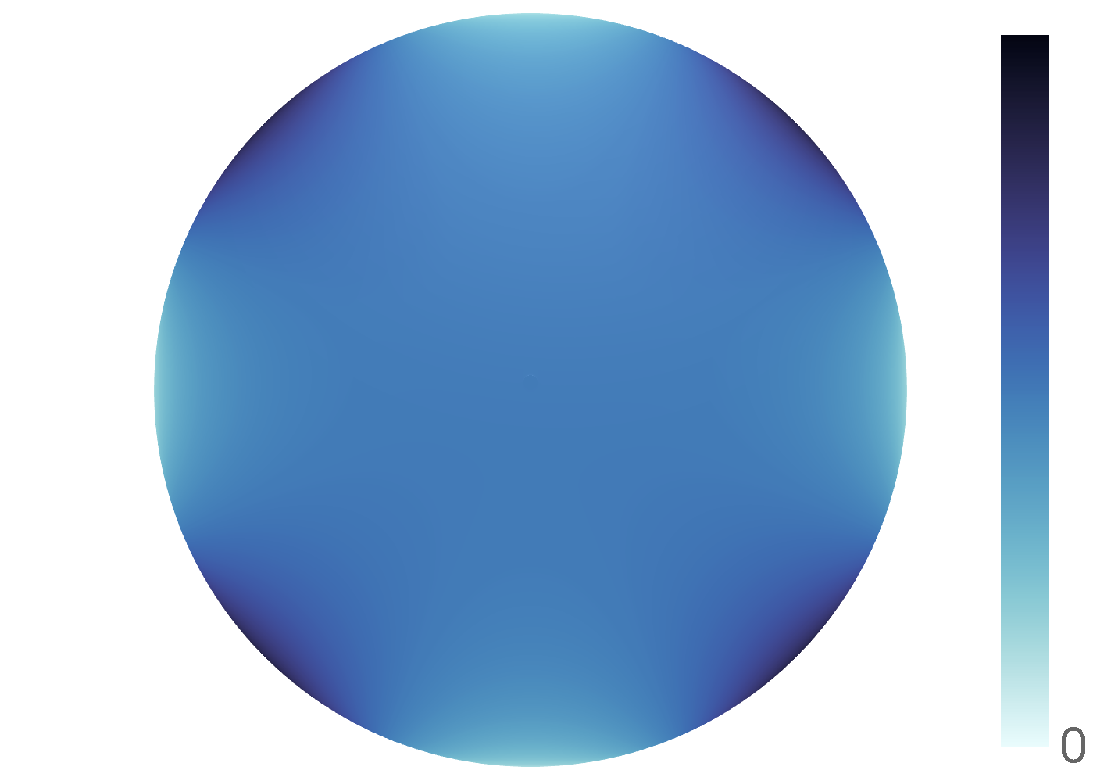
\includegraphics[trim={23 7 3 6},clip,width=.2\textwidth]{spherical_harmonic_4l_4m_L128_real_norm.pdf}}
	\caption[
		The spherical harmonics for \(\ell=0,\ldots,4\)
	]{
		The real part of the spherical harmonics \(\pixel{\harmonic{Y}}\) for \(\ell=0,\ldots,4\) (top-to-bottom) and \(m=0,\ldots,\ell{}\) (left-to-right).
		The negative order harmonics \(\pixel{Y_{\ell(-m)}}\) have not been included as they are simply rotated with respect to the positive order harmonics by \(\SI{90}{\degree}/m\).
	}\label{fig:chapter2_spherical_harmonics}
\end{figure}


\subsection{Rotations on the Sphere}

Rotations of functions defined on the sphere form an integral part of analysis on the sphere.
The Euler angles \(\rho=(\alpha,\beta,\gamma) \in \rotationGroup{}\) may parametrise three-dimensional rotations, where \(\alpha \in \interval[open right]{0}{2\pi}\), \(\beta \in \interval{0}{\pi}\), and \(\gamma \in \interval[open right]{0}{2\pi}\).
The sequence of rotations:
%
\begin{enumerate}[(i),nosep,left=\parindent]
	\item \({\gamma}\) rotation about the \(z\)-axis;
	\item \({\beta}\) rotation about the \(y\)-axis; and
	\item \({\alpha}\) rotation about the \(z\)-axis;
\end{enumerate}
%
define the rotation operator \(\rotation{\rho}\).
A function \(\pixel{f} \in \hilbert{\twoSphere}\) rotated on the sphere is defined by
%
\begin{equation}
	\pixel{(\rotation{\rho}f)}
	%
	= f(\rotationMatrix^{-1} \omega),
\end{equation}
%
where \(\rotationMatrix{}\) is the three-dimensional rotation matrix corresponding to \(\rotation{\rho}\).
A rotation of a spherical harmonic function may be represented by
%
\begin{equation}\label{eq:chapter2_rotate_spherical_harmonics}
	\rotation{\rho} \pixel{\harmonic{Y}}
	%
	= \wignerSum \wigner{\ell}{n}{m}(\rho) \pixel{Y_{\ell n}},
\end{equation}
%
where \(\wigner{\ell}{n}{m}(\rho)\) are the Wigner D matrices~\cite{Brink1993,Ritchie1999}.
The Wigner D matrices form the \(2\ell+1\)-dimensional representation of the rotation group \(\rotationGroup{}\) for a given \(\ell{}\) and are given by
%
\begin{equation}
	\wigner{\ell}{n}{m}(\rho)
	%
	= \exp(-i n\alpha) \reducedWigner{\ell}{n}{m}(\beta) \exp(-i m\gamma),
\end{equation}
%
where \(\reducedWigner{\ell}{n}{m}(\beta)\) are the reduced d matrices which are real in this phase convention and satisfy many symmetry relations.
By the Peter-Weyl theorem, the matrix elements \(\wigner{\ell}{n}{m}(\rho)\) form an orthonormal basis on \(\hilbert{\rotationGroup}\), \ie{}
%
\begin{equation}
	\integrateRotation{\rho} \wigner{\ell}{n}{m}(\rho) \wigner[\ast]{\ell'}{n'}{m'}(\rho)
	%
	= \frac{8\pi^{2}}{2\ell+1} \delta_{\ell\ell'} \delta_{n n'} \delta_{mm'},
\end{equation}
%
where \(\rotationVolume = \sin{\beta}\dd{\alpha}\dd{\beta}\dd{\gamma}\) is the usual invariant measure on \(\rotationGroup{}\).
Similarly, they satisfy the following completeness relation
%
\begin{equation}
	\sum\limits_{\ell=0}^{\infty} \frac{2\ell+1}{8\pi^{2}} \wignerSum \sum\limits_{m=-\ell}^{\ell} \wigner{\ell}{n}{m}(\rho) \wigner[\ast]{\ell}{n}{m}(\rho')
	%
	= \delta(\rho-\rho'),
\end{equation}
%
where
%
\begin{equation}
	\delta(\rho-\rho')
	%
	= \delta(\alpha-\alpha') \delta(\cos{\beta} - \cos{\beta'}) \delta(\gamma-\gamma').
\end{equation}
%
From \cref{eq:chapter2_rotate_spherical_harmonics}, it follows that the harmonic coefficients of a rotated function read
%
\begin{equation}
	\harmonic{(\rotation{\rho}f)}
	%
	= \wignerSum \wigner{\ell}{m}{n}(\rho) f_{\ell n}.
\end{equation}
%
Note the order of the indices on \(\wigner{\ell}{m}{n}(\rho)\) here compared to \cref{eq:chapter2_rotate_spherical_harmonics}.
A function on the rotation group \(F \in \hilbert{\rotationGroup}\) may be represented by an expansion in the Wigner D matrices
%
\begin{equation}
	F(\rho)
	%
	= \sum\limits_{\ell=0}^{\infty} \frac{2\ell+1}{8\pi^{2}} \sum\limits_{m=-\ell}^{\ell} \wignerSum F^{\ell}_{m n} \wigner{\ell}{m}{n}(\rho),
\end{equation}
%
where the Wigner harmonic coefficients \(F^{\ell}_{m n}\) are given by
%
\begin{equation}
	F^{\ell}_{m n}
	%
	= \integrateRotation{\rho} F(\rho) \wigner[\ast]{\ell}{m}{n}(\rho).
\end{equation}
%
A useful relation to note is the connection between the spherical harmonics and the axisymmetric rotation matrices
%
\begin{equation}
	\wigner[\ast]{\ell}{m}{0}(\phi,\theta,0)
	%
	= \sqrt{\inverseFactor} \pixel{\harmonic{Y}}.
\end{equation}

\section{Wavelets}\label{sec:chapter2_wavelets}

Wavelet transforms are ubiquitous in signal processing applications.
In signal analysis, the continuous wavelet transform is more appropriate, \eg{}~\cite{Goupillaud1984,KronlandMartinet1987,Flandrin1989,Holschneider1990,Bertrand1990,Pierce1991}.
Whereas, discrete wavelets and the discrete wavelet transform have greater success in signal coding applications, such as in image compression~\cite{Antonini1990,Mallat1992} and computer vision~\cite{Mallat1989,Shensa1992}.
Presented here is a brief review of wavelet analysis, for more detail see, \eg{}~\cite{Rioul1991,Graps1995,Addison2005,Valens1999,Kaiser2011}.

\subsection{Comparison to the Fourier Transform}\label{sec:chapter2_comparison_fourier_transform}

In Fourier theory, a (Euclidean) signal may be expressed as an infinite sum of sines and cosines.
A significant problem with Fourier analyses, however, is that only the frequency resolutions are known, and not the time resolutions.
Thus, one must seek alternative methods to essentially represent a signal in time and frequency simultaneously.
In these time-frequency joint representations, the idea is to cut the signal into multiple parts and analyse them independently, which can give more detail about the individual frequency components~\cite{Mallat2008}.
Although, making a suitable cut --- which corresponds to a convolution between the signal and the cutting window --- is non-trivial.
Suppose one seeks to find all frequency components present at a given time; naively, this could be achieved by performing a cut with a Dirac delta function.
However, since the Fourier transform of a Dirac delta consists of all possible frequencies (see \cref{fig:chapter2_dirac_fourier}), and a convolution in the time domain corresponds to multiplication in the frequency domain, the signal would be smeared out on the frequency axis.
This problem occurs due to the Heisenberg uncertainty problem; which, in signal processing terms, states that it is impossible to know both the exact frequency, and the exact time of occurrence of this frequency in the signal.

Wavelet analysis is an important signal processing technique which can tackle the shortcomings of the Fourier transform.
A fully scalable, modulated window solves the signal-cutting problem; whereby, the window moves along the signal and a spectrum is calculated at all positions.
After repeating this process multiple times with progressively shorter/longer windows, the end result is a collection of time-frequency representations of the signal, all at different resolutions --- which is often referred to a multiresolution analysis.
\cref{fig:chapter2_ricker_wavelets} presents some example wavelets, Ricker wavelets~\cite{Ricker1953}, where each wavelet is constructed to probe specific frequency ranges.
In wavelet analysis, one typically refers to time-scale (or space-scale) representations, as opposed to time-frequency (like in Fourier theory), where scale is the reciprocal frequency.

\begin{figure}[htpb]
	\centering\capstart{}
	\subfloat[Dirac delta function]
	{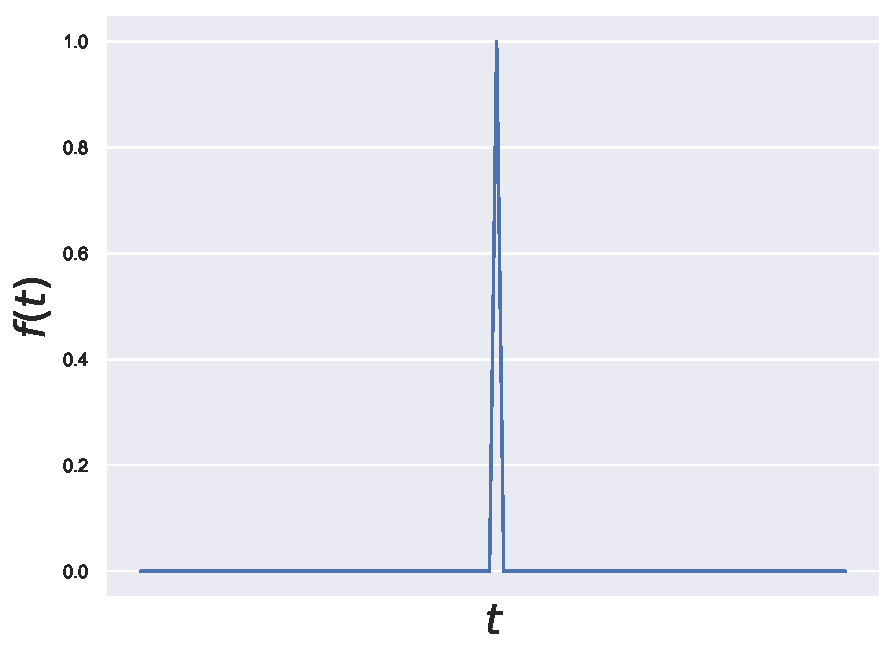
\includegraphics[width=.49\textwidth]{dirac_impulse.pdf}}
	\hfill
	\subfloat[After a Fourier transform]
	{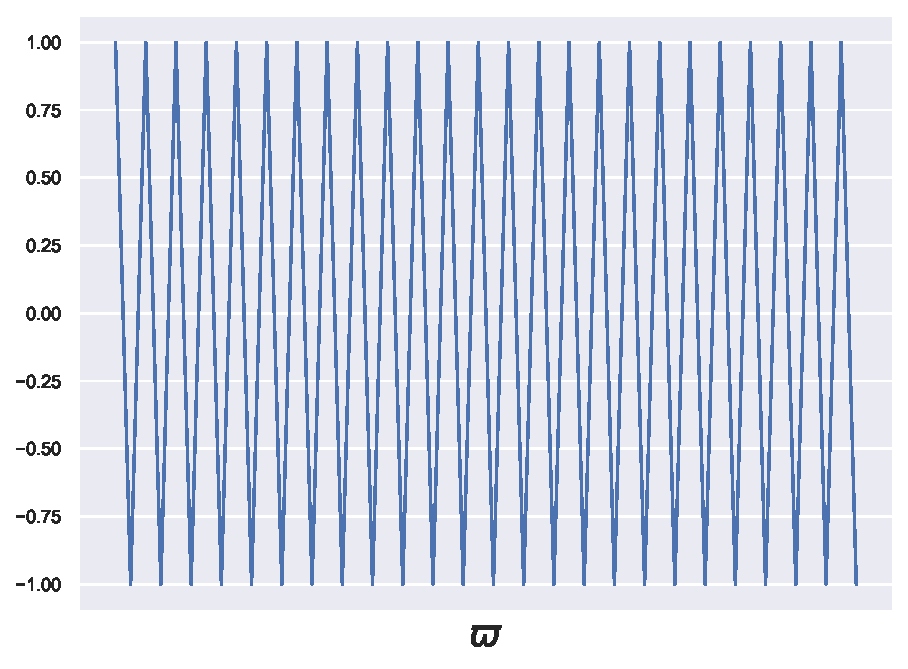
\includegraphics[width=.49\textwidth]{dirac_fft.pdf}}
	\caption[
		A Dirac delta function and the result of a Fourier transform
	]{
		A visual demonstration of the problem with the Fourier transform.
		Panel (a) presents a Dirac delta in the time-domain; which is exactly localised in time, as expected.
		The result of a Fourier transform is shown in panel (b), which now consists of all possible frequencies.
		This phenomenon occurs due to the Heisenberg uncertainty principle.
	}\label{fig:chapter2_dirac_fourier}
\end{figure}


\begin{figure}[htpb]
	\centering\capstart{}
	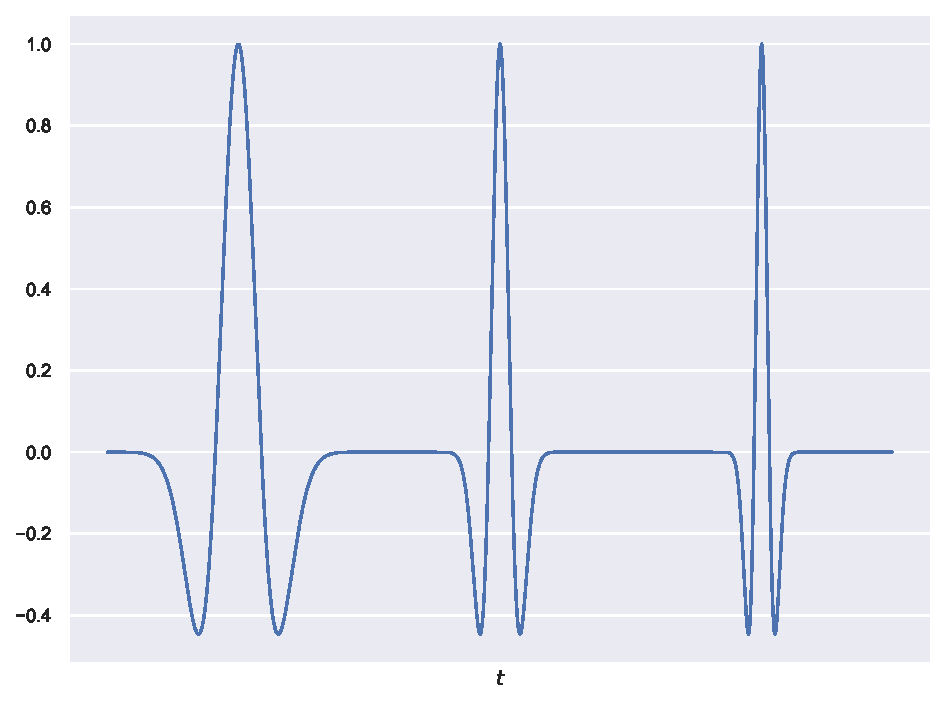
\includegraphics[width=\textwidth]{ricker_wavelets.pdf}
	\caption[
        A few Ricker wavelets
	]{
        Some Ricker wavelets~\cite{Ricker1953} (also known as Mexican hat wavelets) shown alongside each other on the time axis.
        These wavelets arise as the second derivative of the Gaussian function.
        In wavelet analyses, a (Euclidean) signal is probed with many differently sized wavelets.
	}\label{fig:chapter2_ricker_wavelets}
\end{figure}


\subsection{Continuous Wavelet Transform (CWT)}\label{sec:chapter2_continuous_wavelet_transform}

The wavelet analysis described in \cref{sec:chapter2_comparison_fourier_transform} is more formerly known as the CWT, which sates
%
\begin{equation}\label{eq:chapter2_cwt}
	\cwt{f}
	%
	= \int\dd{t} f(t) \Psi^{s\ast}_{\tau}(t),
\end{equation}
%
where \(\Psi^{s}_{\tau}(t)\) are the wavelets, and \(s\) and \(\tau{}\) are dimensionless variables which refer to scale and translation respectively.
\cref{eq:chapter2_cwt} demonstrates how a function \(f(t)\) may be decomposed into a set of wavelets \(\Psi^{s}_{\tau}(t)\) as basis functions.
The inverse wavelet transform is thus
%
\begin{equation}
	f(t)
	%
	= \int\dd{s} \int\dd{\tau} \cwt{f} \Psi^{s}_{\tau}(t).
\end{equation}
%
The wavelets derive from a single wavelet \(\Psi(t)\), the so-called mother wavelet, by scaling and translating, \ie{}
%
\begin{equation}\label{eq:chapter2_mother_wavelet}
	\Psi^{s}_{\tau}(t)
	%
	= \frac{1}{\sqrt{s}} \Psi\bigg(\frac{t-\tau}{s}\bigg),
\end{equation}
%
where the factor \(s^{-1/2}\) is for energy normalisation across different scales.
Here, a general framework has been developed, where the mother wavelet \(\Psi(t)\) is chosen for specific requirements, \eg{} Ricker wavelets are used in seismic wave propagation analyses~\cite{Wang2014}.

\subsection{Wavelet Properties}

The term wavelets arose from the satisfaction of the admissibility and regularity conditions.
The admissibility condition states that the square-integrable functions \(\Psi(t)\) which satisfy
%
\begin{equation}\label{eq:chapter2_admissibility}
	\int\dd{\varpi} \frac{\abs{\fourier{\Psi}(\varpi)}^{2}}{\abs{\varpi}}
	%
	< \infty
\end{equation}
%
can be used to analyse and then reconstruct a signal without loss of information~\cite{Sheng2010}, where \(\fourier{\Psi}(\varpi)\) is the Fourier transform of the wavelet \(\Psi(t)\).
Therefore, \cref{eq:chapter2_admissibility} implies that the Fourier transform of the wavelet vanishes at zero frequency, \ie{}
%
\begin{equation}
	\abs{\fourier{\Psi}(\varpi)} \bigg\rvert_{\varpi=0}
	%
	= 0;
\end{equation}
%
which means the spectrum experiences bandpass behaviour.
It also follows that, the average value of the wavelet in the time-domain must be zero, \ie{}
%
\begin{equation}
	\int\dd{t} \Psi(t)
	%
	= 0,
\end{equation}
%
which indicates that it must be an oscillatory function (a wave).
Regularity conditions are imposed such that the wavelets are somewhat smooth and concentrated in both time and frequency.
In \cref{eq:chapter2_cwt}, the wavelet transform of a one-dimensional function \(f(t)\) is two-dimensional --- and a two-dimensional function would have a four-dimensional transform \etc{}
Moreover, the square of the input signal is the time-bandlimit product of the wavelet transform.
Thus, some extra constraints are imposed on the wavelets such that they decrease rapidly as the scale \(s\) decreases.
For more detail on regularity see~\cite{Burrus1997,Daubechies1992}.

\subsection{Discrete Wavelets}\label{sec:chapter2_discrete_wavelets}

In practice, the CWT described in \cref{sec:chapter2_continuous_wavelet_transform} is impractical to use: namely, the wavelet transform \cref{eq:chapter2_cwt} is redundant, \ie{} the scaled functions do not form an orthogonal basis; the CWT has an infinite number of wavelets in the wavelet transform; and, most wavelet transforms do not have analytical solutions and hence must be computed numerically.
Discrete wavelets overcome these problems by modifying the continuous wavelet \cref{eq:chapter2_mother_wavelet} by
%
\begin{equation}\label{eq:chapter2_discrete_wavelets}
	\Psi^{j}_{\lambda}(t)
	%
	= \frac{1}{\sqrt{s^{j}_{0}}} \Psi\Bigg(\frac{t - \lambda\tau_{0}s^{j}_{0}}{s^{j}_{0}}\Bigg),
\end{equation}
%
where \(j\) and \(\lambda{}\) are integers, \(s_{0}>1\) is a fixed dilation step, and \(\tau_{0}\) is the translation factor.
Thus, discrete wavelets may only be scaled and translated in discrete steps.
Discrete wavelets are used to transform a continuous signal into a series of wavelet coefficients, known as a wavelet decomposition.
A natural choice for the parameters in \cref{eq:chapter2_discrete_wavelets} are \(s_{0}=2\) and \(\tau_{0}=1\) which corresponds to dyadic scaling, the discrete wavelets are thus
%
\begin{equation}
	\Psi^{j}_{\lambda}(t)
	%
	= 2^{-j/2} \Psi(2^{-j}t - \lambda).
\end{equation}
%
A necessary and sufficient condition for stable signal reconstruction is the so-called Parseval frame property
%
\begin{equation}
	A \norm{f}^{2}
	%
	\leq \sum\limits_{j} \sum\limits_{\lambda} \abs{\braket*{f}{\Psi^{j}_{\lambda}}}^{2}
	%
	\leq B \norm{f}^{2},
\end{equation}
%
with \(A,\ B \in \realPosParam{}\)~\cite{Daubechies1992}.
When \(A=B=1\) the energy of \(f\) is conserved in wavelet space, and as such the wavelets act like an orthonormal basis, \ie{}
%
\begin{equation}
	\int\dd{t} \Psi^{j}_{\lambda}(t) \Psi^{j'\ast}_{\lambda'}(t)
	%
	= \delta_{j j'} \delta_{\lambda\lambda'},
\end{equation}
%
which solves the redundancy problem.
Therefore, a signal may be constructed by~\cite{Sheng2010}
%
\begin{equation}
	f(t)
	%
	= \sum\limits_{j} \sum\limits_{\lambda} W^{j}_{\lambda} \Psi^{j}_{\lambda}(t),
\end{equation}
%
where \(W^{j}_{\lambda}\) are the wavelet coefficients given by
%
\begin{equation}
	W^{j}_{\lambda}
	%
	= \int\dd{t} f(t) \Psi^{j\ast}_{\lambda}(t).
\end{equation}
%
To get good coverage with a finite number of wavelets, a logarithmic tiling of Fourier space (\ie{} scale) is used to construct the wavelets, such as in \cref{fig:chapter2_tiling}.
A scaling function \(\Phi_{\lambda}(t)\), in blue, is typically introduced to capture the lower scales of the underlying function~\cite{Mallat1989}.

\subsection{Discrete Wavelet Transform (DWT)}

The discrete wavelets introduced in \cref{sec:chapter2_discrete_wavelets} are discretised in translation and scale, but not in time.
In reality, most signals of interest are sampled, and are in fact not time-continuous.
Thus, the CWT described in \cref{sec:chapter2_continuous_wavelet_transform} becomes
%
\begin{equation}
	\text{DWT}_{f}(j,\lambda)
	%
	= \sum\limits_{i} f[t_{i}] \Psi^{j\ast}_{\lambda}[t_{i}],
\end{equation}
%
where a sum replaces the integral in \cref{eq:chapter2_cwt}.
Upon introduction of a scaling function (to capture the lower scales), a signal may be reconstructed from its scaling/wavelet coefficients by
%
\begin{equation}
	f(t)
	%
	= \sum\limits_{i} \sum\limits_{\lambda} W^{\Phi}_{\lambda} \Phi_{\lambda}[t_{i}]
	%
	+ \sum\limits_{j} W^{\Psi^{j}}_{\lambda} \Psi^{j}_{\lambda}[t_{i}],
\end{equation}
%
where the scaling coefficients (and similarly for the wavelet coefficients \(W^{\Psi^{j}}_{\lambda}\)) are found by
%
\begin{equation}
	W^{\Phi}_{\lambda}
	%
	= \sum\limits_{i} f[t_{i}] \conj{\Phi}_{\lambda}[t_{i}].
\end{equation}
%
Fast algorithms exist~\cite{Beylkin1991,Rioul1992}, in which recursion relations allow one to compute the wavelet at scale \(j+1\) from scale \(j\).

\subsection{Extension to the Sphere}

Whilst wavelet theory was initially considered in the Euclidean domain, it has since been generalised to the sphere in both the continuous~\cite{Torresani1995,Holschneider1996,Freeden1997,Antoine1998,Antoine1999,Antoine2002,Demanet2003,Wiaux2005,Sanz2006,McEwen2006} and discrete~\cite{Sweldens1996,Schroder2000,Wiaux2005,Starck2006,Wiaux2008,Starck2009,Leistedt2013,McEwen2019,McEwen2018} settings.
Few wavelet frameworks on the sphere have exact transforms in both settings.
Scale-discretised wavelets~\cite{Wiaux2008,McEwen2018,Leistedt2013,McEwen2013,McEwen2015} are such a framework, which lean on a tiling of the (spherical) harmonic line to produce the wavelet transform.
\cref{fig:chapter2_axisymmetric_wavelets} presents some example axisymmetric scale-discretised wavelets on the sphere, constructed from the tiling shown in \cref{fig:chapter2_tiling}.
Here, the parameter combination \(\lambda=3\), \(J_{0}=2\) and bandlimit \(L=128\) results in a scaling function in panel (a) and four wavelets shown in panels (b-e).
Much like in the Euclidean setting, a signal (on the sphere) is probed by multiple wavelets at different scales such as these.

\begin{figure}[htpb]
	\centering\capstart{}
	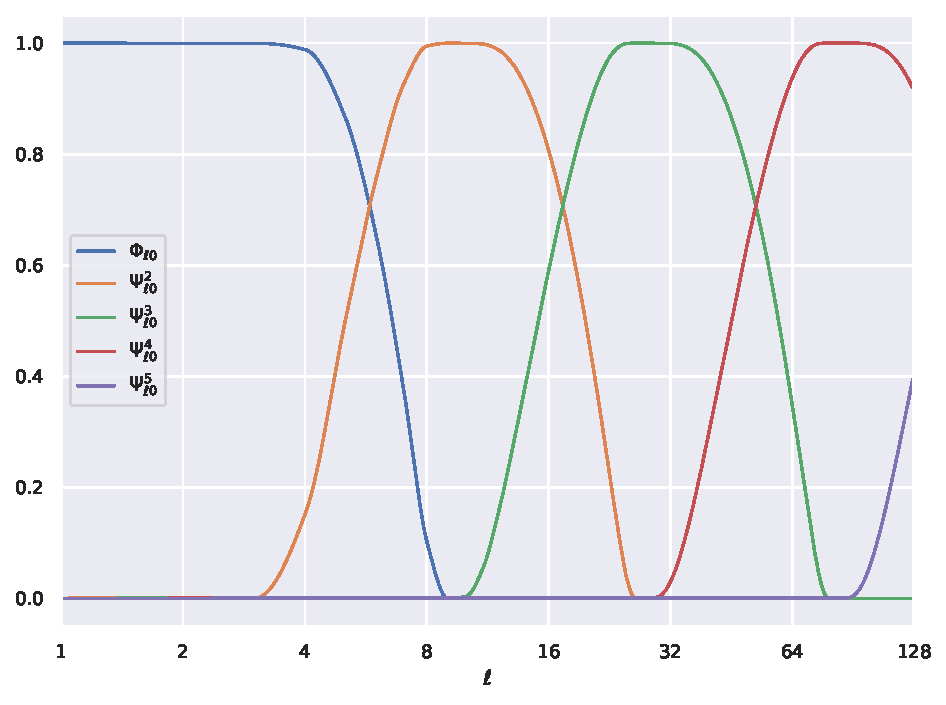
\includegraphics[width=\textwidth]{axisymmetric_tiling_L128.pdf}
	\caption[
	]{
	}\label{fig:chapter2_tiling}
\end{figure}


\begin{figure}[htpb]
	\centering\capstart{}
	\subfloat[\(\pixel{\Phi}\)]
	{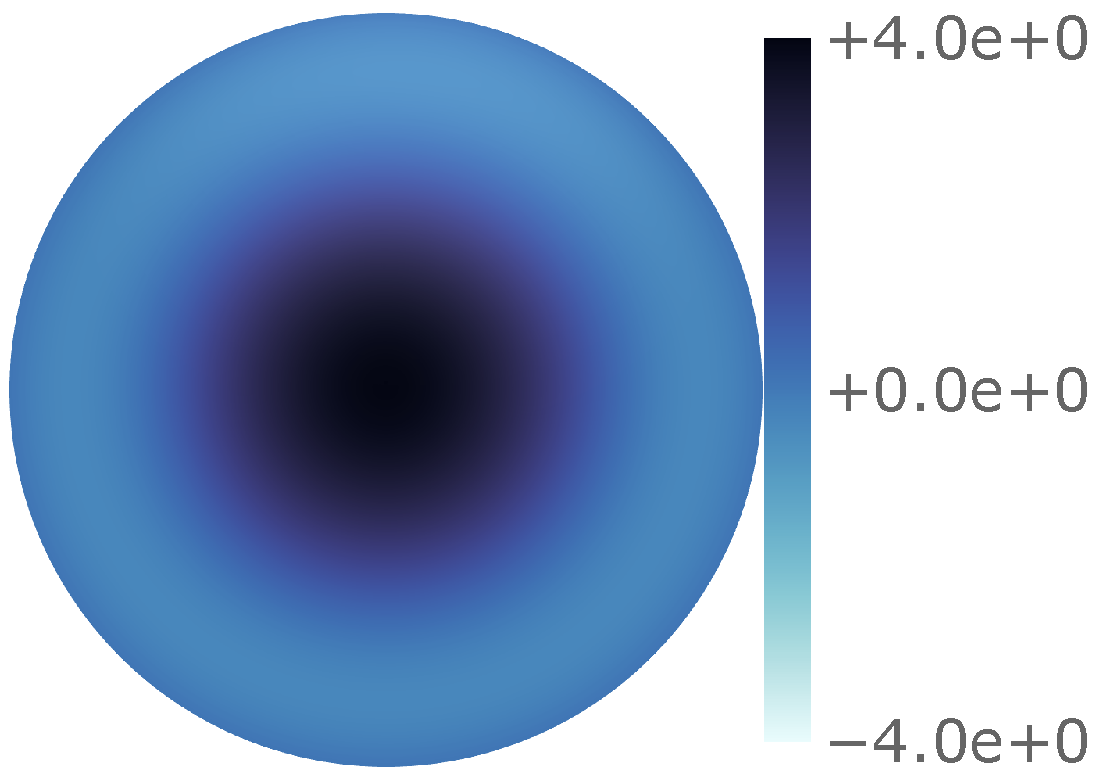
\includegraphics[trim={4 7 3 6},clip,width=.33\textwidth]{axisymmetric_wavelets_3B_2jmin_scaling_L128_res512_real.pdf}}
	\hfill
	\subfloat[\(\pixel{\Psi^{2j}}\)]
	{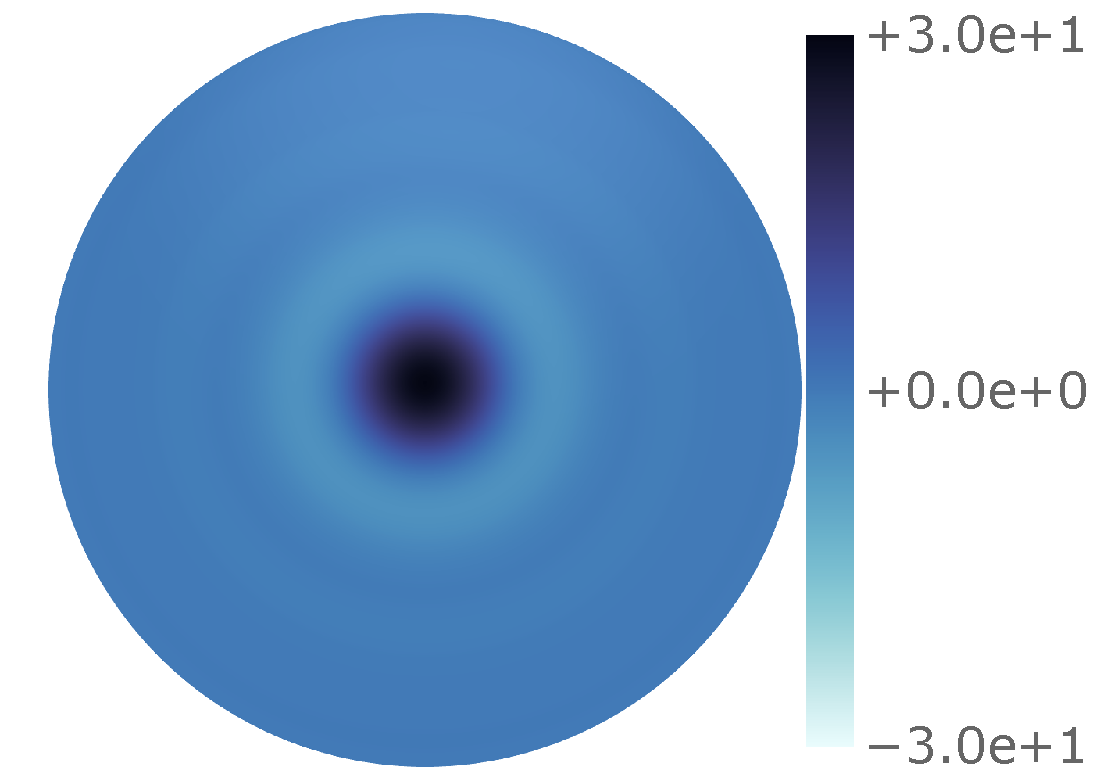
\includegraphics[trim={4 7 3 6},clip,width=.33\textwidth]{axisymmetric_wavelets_3B_2jmin_2j_L128_res512_real.pdf}}
	\hfill
	\subfloat[\(\pixel{\Psi^{3j}}\)]
	{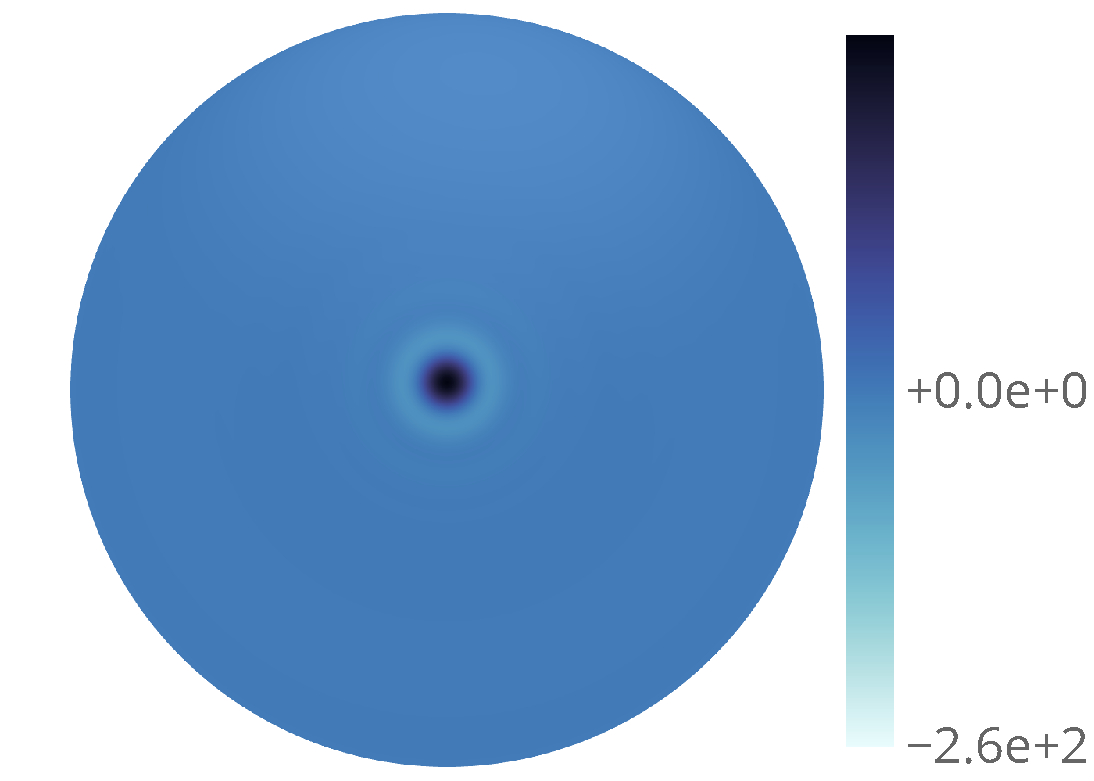
\includegraphics[trim={4 7 3 6},clip,width=.33\textwidth]{axisymmetric_wavelets_3B_2jmin_3j_L128_res512_real.pdf}}
	\newline
	\subfloat[\(\pixel{\Psi^{4j}}\)]
	{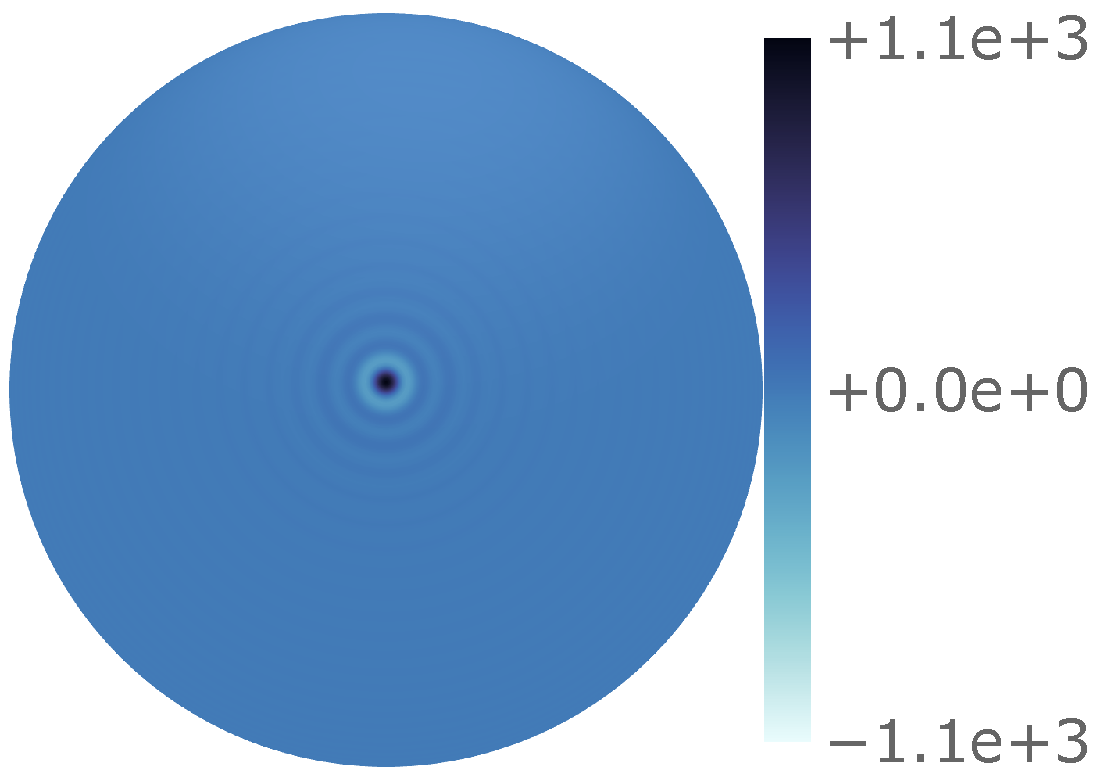
\includegraphics[trim={4 7 3 6},clip,width=.33\textwidth]{axisymmetric_wavelets_3B_2jmin_4j_L128_res512_real.pdf}}
	%
	\subfloat[\(\pixel{\Psi^{5j}}\)]
	{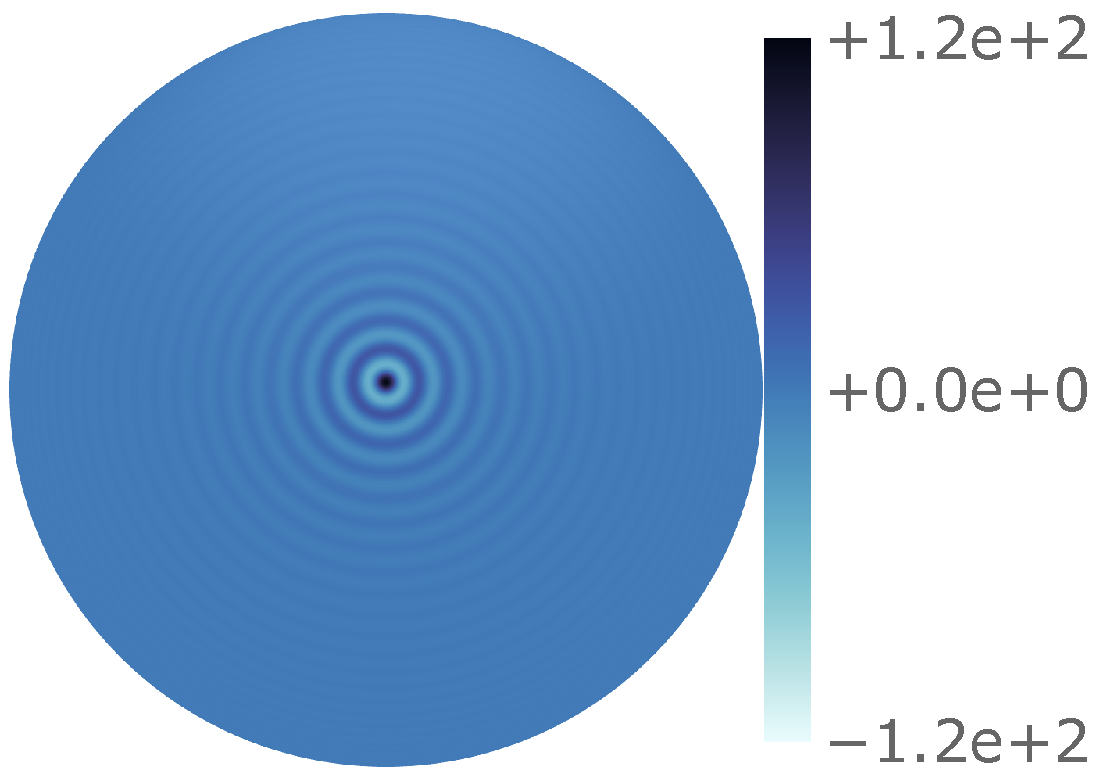
\includegraphics[trim={4 7 3 6},clip,width=.33\textwidth]{axisymmetric_wavelets_3B_2jmin_5j_L128_res512_real.pdf}}
	\caption[
		Some axisymmetric scale-discretised wavelets on the sphere
	]{
		The scaling function and the wavelets for scales \(j \in \set{2, 3, 4, 5}\) of the axisymmetric scale-discretised wavelets on the sphere centred on the north pole shown left-to-right, top-to-bottom.
		They are constructed through a tiling of the harmonic line with parameters \(\lambda=3\), \(J_{0}=2\), and bandlimit \(L=128\) (\cf{} \cref{fig:chapter2_tiling}).
	}\label{fig:chapter2_axisymmetric_wavelets}
\end{figure}


\section{Slepian Concentration Problem}\label{sec:chapter2_slepian_concentration_problem}

In the 1960s, Slepian, Landau and Pollak solved the fundamental problem of optimally concentrating a signal simultaneously in time and frequency~\cite{Landau1961,Landau1962,Slepian1983,Slepian1961}.
The resulting orthogonal family of functions, and their discrete and multidimensional counterparts~\cite{Bronez1988,Hanssen1997,Liu1992,Slepian1964,Slepian1978}, form the basis of a range of spectral analyses (\eg{}~\cite{Thomson1982,Thomson1990}).
In contrast to wavelets, described in \cref{sec:chapter2_wavelets}, the so-called Slepian functions allow one to compute localised spatial-spectral analysis, as opposed to spatial-scale.
\cref{sec:chapter2_slepian_euclidean} follows with a brief review of the initial time-frequency concentration problem, this is then extended to the spherical domain in \cref{sec:chapter2_slepian_sphere}.

\subsection{Time-Frequency Domain}\label{sec:chapter2_slepian_euclidean}

Before considering the Slepian spatial-spectral concentration problem in the spherical domain, first consider the one-dimensional, continuous-continuous, time-frequency concentration problem.
Here, a normalisation convention is adopted such that a real-valued time-domain single \(f(t)\) and its Fourier transform \(\fourier{f}(\varpi)\) are related by
%
\begin{equation}\label{eq:chapter2_fourier_time}
	f(t)
	%
	= \frac{1}{2\pi} \int\limits_{-\infty}^{\infty} \dd{\varpi} \fourier{f}(\varpi) \exp(i\varpi t)
\end{equation}
%
and
%
\begin{equation}\label{eq:chapter2_fourier_frequency}
	\fourier{f}(\varpi)
	%
	= \int\limits_{-\infty}^{\infty} \dd{\varpi} f(t) \exp(-i\varpi t),
\end{equation}
%
where \(t\) and \(\varpi{}\) denote the time and angular frequency respectively.
Slepian and Pollak~\cite{Slepian1961} considered the problem of optimally concentrating a strictly bandlimited signal \(f(t)\), with a spectrum \(\fourier{f}(\varpi)\) which vanishes into a time interval \(\abs{t} \leq T\) for frequencies \(\abs{\varpi} > W\).
Through the Paley-Wiener theorem, no bandlimited signal \(g(t)\) can be exactly concentrated within a finite interval~\cite{Daubechies1992,Mallat2008}.
To find the optimally concentrated signal, one must maximise the following ratio
%
\begin{equation}\label{eq:chapter2_frequency_ratio}
	\mu
	%
	= \frac{\displaystyle\int\limits_{-T}^{T} \dd{t} \abs{g(t)}^{2}}
	%
	{\displaystyle\int\limits_{-\infty}^{\infty} \dd{t} \abs{g(t)}^{2}},
\end{equation}
%
although other criteria have been considered~\cite{Freeden1997,Riedel1995}.
Bandlimited signals \(g(t)\) which satisfy \cref{eq:chapter2_frequency_ratio}, have spectra \(\fourier{g}(\varpi)\) which satisfy the convolutional integral eigenproblem in the frequency-domain
%
\begin{equation}\label{eq:chapter2_frequency_eigenproblem}
	\int\limits_{-W}^{W} \dd{\varpi'} \frac{\sin{T(\varpi-\varpi')}}{\pi(\varpi-\varpi')} \fourier{g}(\varpi')
	%
	= \mu \fourier{g}(\varpi),
\end{equation}
%
where \(\abs{\varpi} \leq W\).

Slepian \etal{} also considered the similar case of concentrating the spectrum \(\fourier{h}(\varpi)\) of a strictly timelimited function \(h(t)\), which vanishes into a spectral interval \(\abs{\varpi} \leq W\) for times \(\abs{t} > T\).
The ratio to maximise here is
%
\begin{equation}\label{eq:chapter2_time_ratio}
	\mu
	%
	= \frac{\displaystyle\int\limits_{-W}^{W} \dd{\varpi} \abs{\fourier{h}(\varpi)}^{2}}
	%
	{\displaystyle\int\limits_{-\infty}^{\infty} \dd{\varpi} \abs{\fourier{h}(\varpi)}^{2}},
\end{equation}
%
which results in the time-domain eigenproblem
%
\begin{equation}\label{eq:chapter2_time_eigenproblem}
	\int\limits_{-T}^{T} \dd{t'} \frac{\sin{W(t-t')}}{\pi(t-t')} h(t')
	%
	= \mu h(t),
\end{equation}
%
where \(\abs{t} < T\).
In either case, the eigenvalues (which represent effective concentration) satisfy
%
\begin{equation}
	1 > \mu_{1} \geq \mu_{2} \geq \ldots > 0, % chktex 11
\end{equation}
%
with associated eigenfunctions, \eg{}
%
\begin{equation}
	g_{1}(t),\ g_{2}(t),\ \ldots
\end{equation}
%
which exist in the interval \(\abs{t} \leq T\).
Through a change of variables, the ratios \cref{eq:chapter2_frequency_ratio,eq:chapter2_time_ratio} may be transformed into one dimensionless eigenproblem
%
\begin{equation}
	\int\limits_{-1}^{1} \dd{y} \frac{\sin{TW(x-y)}}{\pi(x-y)} \zeta(y)
	%
	= \mu \zeta(x),
\end{equation}
%
where \(\abs{x} \leq 1\).
Hence, the eigenvalues and scaled eigenfunctions only depend on the time-bandlimit product \(TW\).
Consider the sum of the eigenvalues
%
\begin{equation}
	N
	%
	= \sum\limits_{p=1}^{\infty} \mu_{p}
	%
	= \frac{2TW}{\pi}.
\end{equation}
%
The so-called Shannon number~\cite{Percival1993} \(N\) introduced here is a good estimate of the number of significant eigenvalues, which arises due to the characteristic shape of the eigenvalue spectrum~\cite{Landau1965,Slepian1965} (see \cref{fig:chapter2_polar_cap_eigenvalues}).
Equivalently, this can be viewed as the number of signals \(f(t)\) which can be well-concentrated both into a finite time interval \(\abs{t} \leq T\) and a finite frequency interval \(\abs{\varpi} \leq W\).
Many of the results discussed above have analogues in the spatial-spectral concentration problem on the sphere, which is elaborated in \cref{sec:chapter2_slepian_sphere}.

\subsection{Spatial-Spectral Domain}\label{sec:chapter2_slepian_sphere}

The two sub-spaces of interest of all square-integrable functions on the sphere \(\twoSphere{}\) are: \(\spaceSpacelimit{}\) the space of all spacelimited functions strictly contained within a region \(R\), and \(\spaceBandlimit{}\) the space of all bandlimited functions with no power above the bandlimit \(L\).
Akin to the Euclidean setting, no function can be strictly spacelimited as well as strictly bandlimited, \ie{} no \(\pixel{f}\) can be in both sub-spaces \(\spaceSpacelimit{}\) and \(\spaceBandlimit{}\) at the same time.
Thus, one may find either: the spacelimited functions \(\pixel{h} \in \spaceSpacelimit{}\) whose spectrum is optimally concentrated within the interval \(0 \leq \ell < L\), or the bandlimited functions \(\pixel{g} \in \spaceBandlimit{}\) which are optimally concentrated within a region \(R\).

\subsubsection{Spectral Concentration of a Spacelimited Function}

To maximise the concentration of a spacelimited function \(\pixel{h} \in \spaceSpacelimit{}\) within an interval \(0 \leq \ell < L\) one must maximise the ratio
%
\begin{equation}\label{eq:chapter2_spacelimited_ratio}
	\mu
	%
	= \frac{\displaystyle\sum\limits_{\ell=0}^{L-1} \sum\limits_{m=-\ell}^{\ell} \abs{\harmonic{h}}^{2}}
	%
	{\displaystyle\sum\limits_{\ell=0}^{\infty} \sum\limits_{m=-\ell}^{\ell} \abs{\harmonic{h}}^{2}},
\end{equation}
%
which is analogous to the one-dimensional problem \cref{eq:chapter2_time_ratio}.
By substituting the expansion of the spherical harmonic coefficients
%
\begin{equation}
	\harmonic{h}
	%
	= \integrateRegion{\sphereVolume} \pixel{h} \pixel{\conj{\harmonic{Y}}},
\end{equation}
%
and swapping the order of summation and integration, the variational problem \cref{eq:chapter2_spacelimited_ratio} becomes
%
\begin{equation}
	\mu
	%
	= \frac{\integrateRegion{\sphereVolume[']} \pixel[']{h} \integrateRegion{\sphereVolume} \pixel{\delta_{\omega'}} \pixel{\conj{h}}}
	%
	{\integrateRegion{\sphereVolume} \abs{\pixel{h}}^{2}},
\end{equation}
%
where
%
\begin{equation}
	\pixel{\delta_{\omega'}}
	%
	= \sum\limits_{\ell=0}^{L-1} \sum\limits_{m=-\ell}^{\ell} \pixel[']{\conj{\harmonic{Y}}} \pixel{\harmonic{Y}}
\end{equation}
%
is the bandlimited Dirac delta function.
The maximally spacelimited functions \(\pixel{h} \in \spaceSpacelimit{}\) are therefore the solutions to the integral equation
%
\begin{equation}
	\integrateRegion{\sphereVolume} \pixel{\delta_{\omega'}} \pixel{\conj{h}}
	%
	= \mu \pixel[']{\conj{h}},
\end{equation}
%
which is the spherical analogue of the one-dimensional time-domain eigenproblem \cref{eq:chapter2_time_eigenproblem}.

\subsubsection{Spatial Concentration of a Bandlimited Function}\label{sec:chapter2_spatial_concentration_bandlimited_function}

Conversely, to find the maximally concentrated bandlimited functions \(\pixel{g} \in \spaceBandlimit{}\) within a region \(R\) one must maximise the ratio
%
\begin{equation}\label{eq:chapter2_bandlimited_ratio}
	\mu
	%
	= \frac{\integrateRegion{\sphereVolume} \abs{\pixel{g}}^{2}}
	%
	{\integrateSphere{\omega} \abs{\pixel{g}}^{2}},
\end{equation}
%
which is, as before, analogous to the one-dimensional problem \cref{eq:chapter2_frequency_ratio}.
Expanding in harmonic space, and swapping the order of summation and integration, \cref{eq:chapter2_bandlimited_ratio} becomes
%
\begin{equation}
	\mu
	%
	= \frac{\displaystyle\sum\limits_{\ell=0}^{L-1} \sum\limits_{m=-\ell}^{\ell} \harmonic{g}
		%
		\sum\limits_{\ell'=0}^{L-1} \sum\limits_{m'=-\ell'}^{\ell'} \Dmatrix \conj{\harmonic[']{g}}}
	%
	{\displaystyle\sum\limits_{\ell=0}^{L-1} \sum\limits_{m=-\ell}^{\ell} \abs{\harmonic{g}}^{2}},
\end{equation}
%
where
%
\begin{equation}
	\Dmatrix
	%
	= \integrateRegion{\sphereVolume} \pixel{\harmonic{Y}} \pixel{\conj{\harmonic[']{Y}}}
\end{equation}
%
is an \(L \times L\) matrix.
The eigenproblem, of which the maximally bandlimited functions derive from, is
%
\begin{equation}
	\sum\limits_{\ell'=0}^{L-1} \sum\limits_{m'=-\ell'}^{\ell'} \Dmatrix \conj{\harmonic[']{g}}
	%
	= \mu \conj{\harmonic{g}},
\end{equation}
%
which is analogous to the one-dimensional frequency-domain eigenproblem \cref{eq:chapter2_frequency_eigenproblem}.

To explore this further, consider the straightforward case of finding the maximally concentrated functions within an axisymmetric polar cap of colatitudinal radius \(\theta_{0}\), centred on the north pole, \ie{}
%
\begin{equation}
	R
	%
	= \set{\theta: 0 \leq \theta \leq \theta_{0}}.
\end{equation}
%
\cref{fig:chapter2_slepian_polar_cap} presents the first sixteen Slepian functions \(\pixel{\slepian{S}}\) for a colatitude \(\theta_{0}=\SI{40}{\degree}\) and bandlimit \(L=16\).
The Shannon number is \(N=30\) for this region and bandlimit, and therefore all Slepian functions shown are well-concentrated within the region --- as shown by the eigenvalues \(\mu_{p}\), which are all \(\almost{1}\).
Visually, these polar cap Slepian functions look like the spherical harmonics (\cf{} \cref{fig:chapter2_spherical_harmonics}); where the number of positive/negative regions relates to the order \(m\) in the submatrix \(D_{\ell m,\ell'm}\).
The colatitudinal dependence is examined (by keeping \(\phi{}\) constant) for this region in \cref{fig:chapter2_slepian_colatitude} for \(p \in \set{1,6,15,30,51,72}\) shown left-to-right, top-to-bottom.
For the early \(p\) values the majority of the power of the signal is in the blue curve; however, by the final plot, most of the content of the signal is in the orange curve.
The corresponding eigenvalues \(\mu_{p}\) for this region are given in \cref{fig:chapter2_polar_cap_eigenvalues}, whereby the characteristic step shape around the Shannon number is observed.

\begin{figure}[htpb]
	\centering\capstart{}
	\subfloat[\(\mu_{1}=1.000000\)]
	{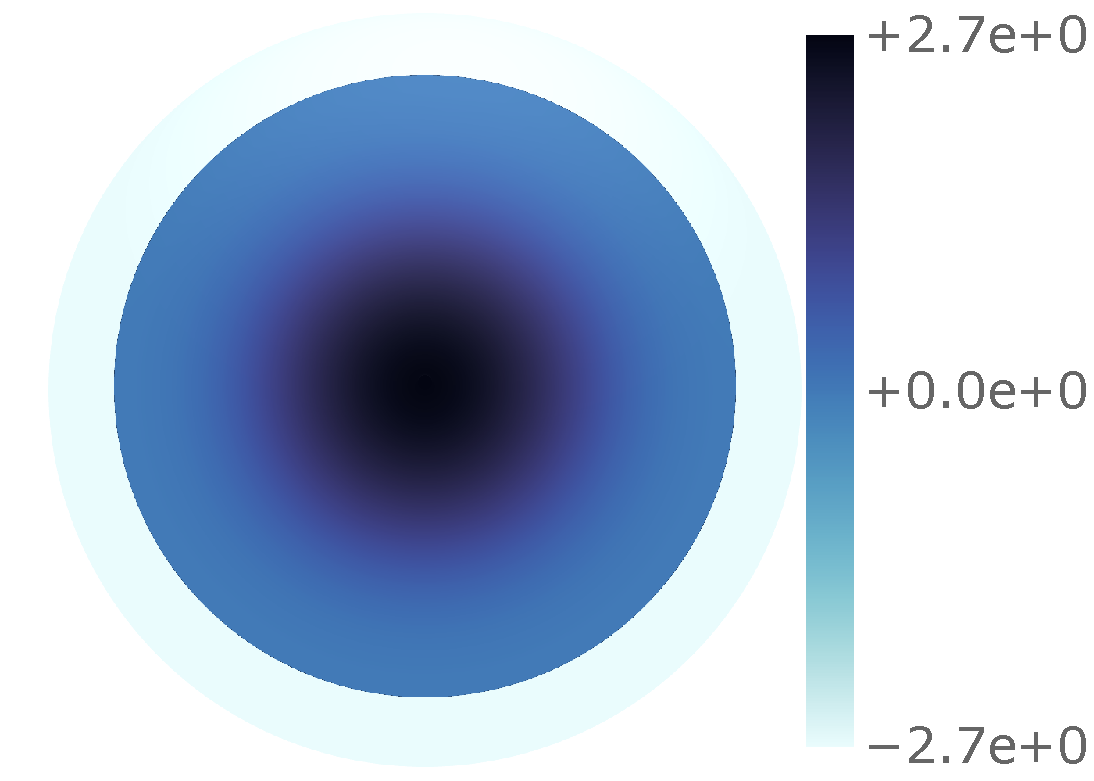
\includegraphics[trim={23 7 3 6},clip,width=.25\textwidth]{slepian_polar40_m0_rank0_lam1-000000e00_L16_res128_real.pdf}} % chktex 8
	\hfill
	\subfloat[\(\mu_{2}=0.999998\)]
	{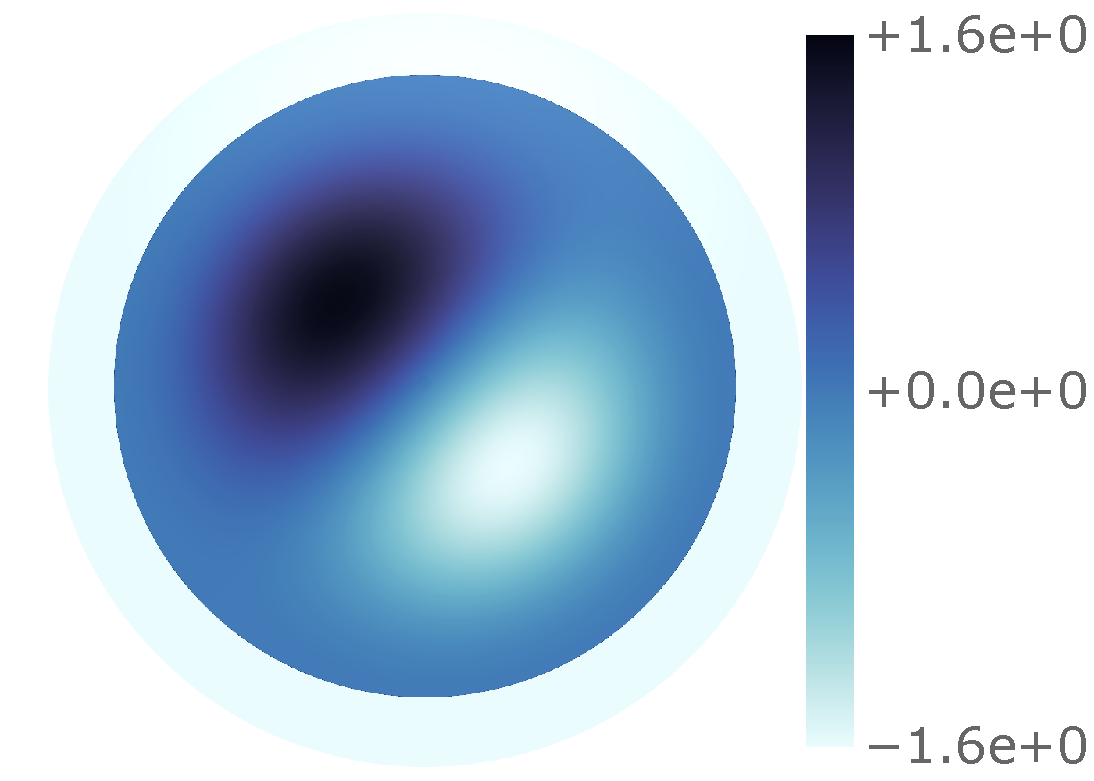
\includegraphics[trim={23 7 3 6},clip,width=.25\textwidth]{slepian_polar40_m-1_rank1_lam9-999984e-01_L16_res128_real.pdf}} % chktex 8
	\hfill
	\subfloat[\(\mu_{3}=0.999998\)]
	{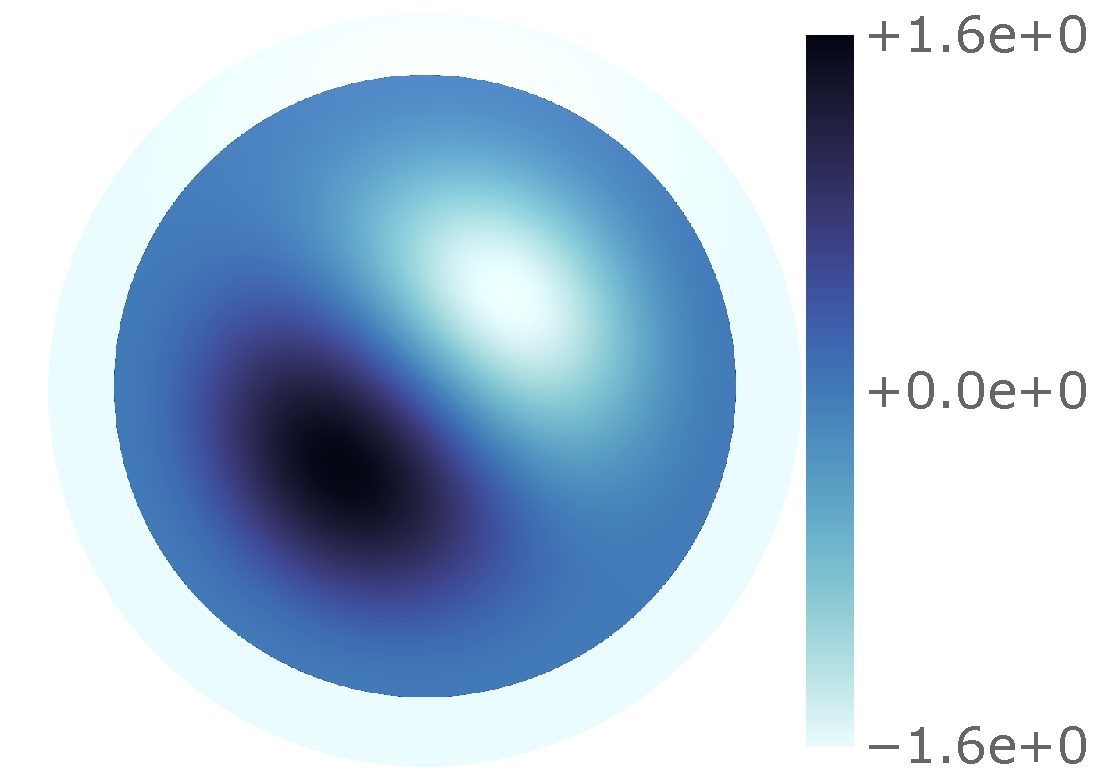
\includegraphics[trim={23 7 3 6},clip,width=.25\textwidth]{slepian_polar40_m1_rank2_lam9-999984e-01_L16_res128_real.pdf}} % chktex 8
	\hfill
	\subfloat[\(\mu_{4}=0.999966\)]
	{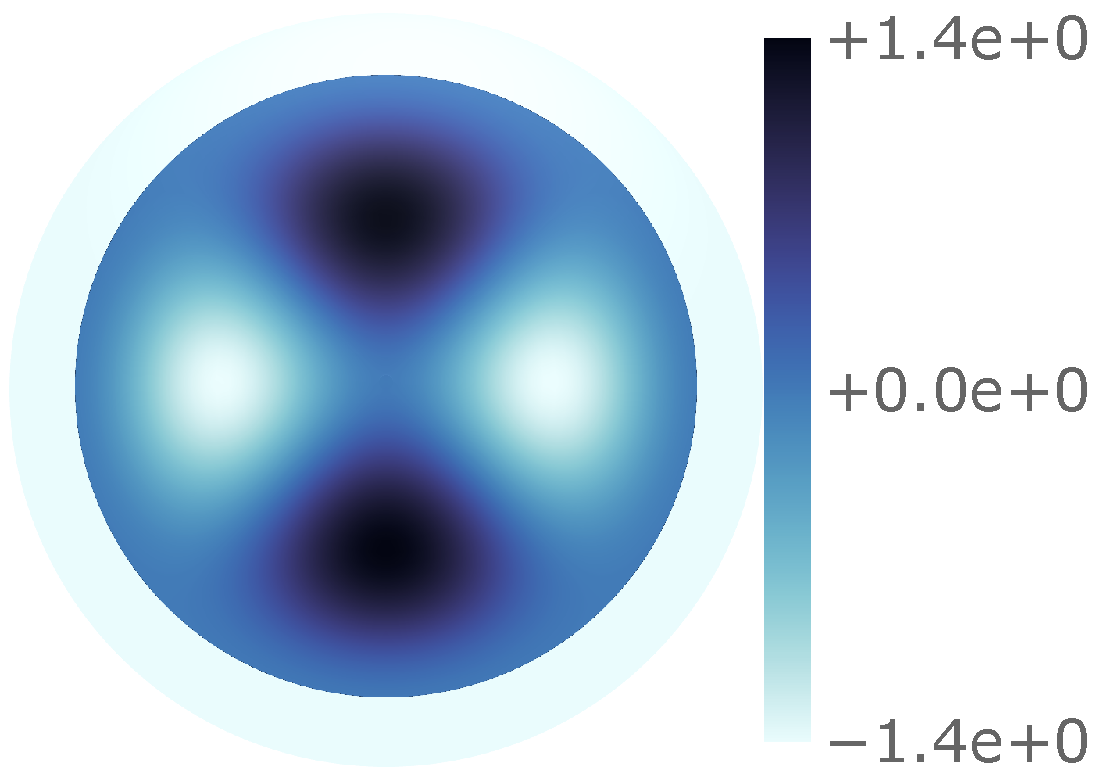
\includegraphics[trim={23 7 3 6},clip,width=.25\textwidth]{slepian_polar40_m-2_rank3_lam9-999664e-01_L16_res128_real.pdf}} % chktex 8
	\newline
	\subfloat[\(\mu_{5}=0.999966\)]
	{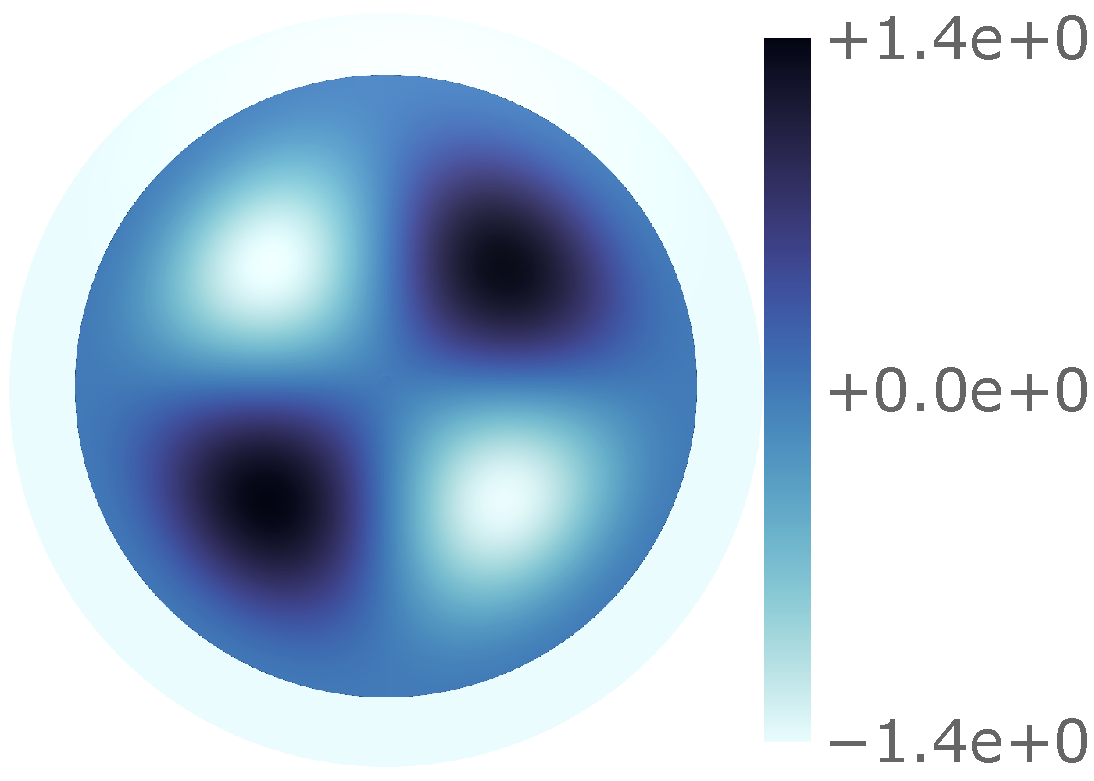
\includegraphics[trim={23 7 3 6},clip,width=.25\textwidth]{slepian_polar40_m2_rank4_lam9-999664e-01_L16_res128_real.pdf}} % chktex 8
	\hfill
	\subfloat[\(\mu_{6}=0.999939\)]
	{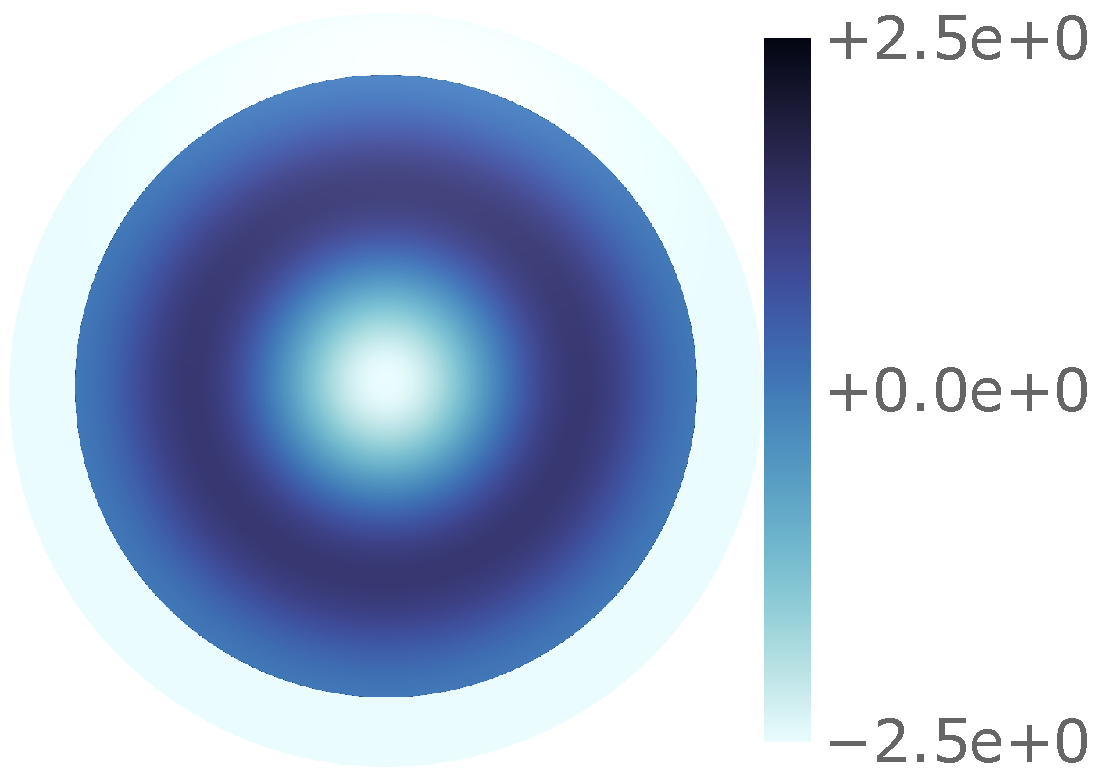
\includegraphics[trim={23 7 3 6},clip,width=.25\textwidth]{slepian_polar40_m0_rank5_lam9-999392e-01_L16_res128_real.pdf}} % chktex 8
	\hfill
	\subfloat[\(\mu_{7}=0.999553\)]
	{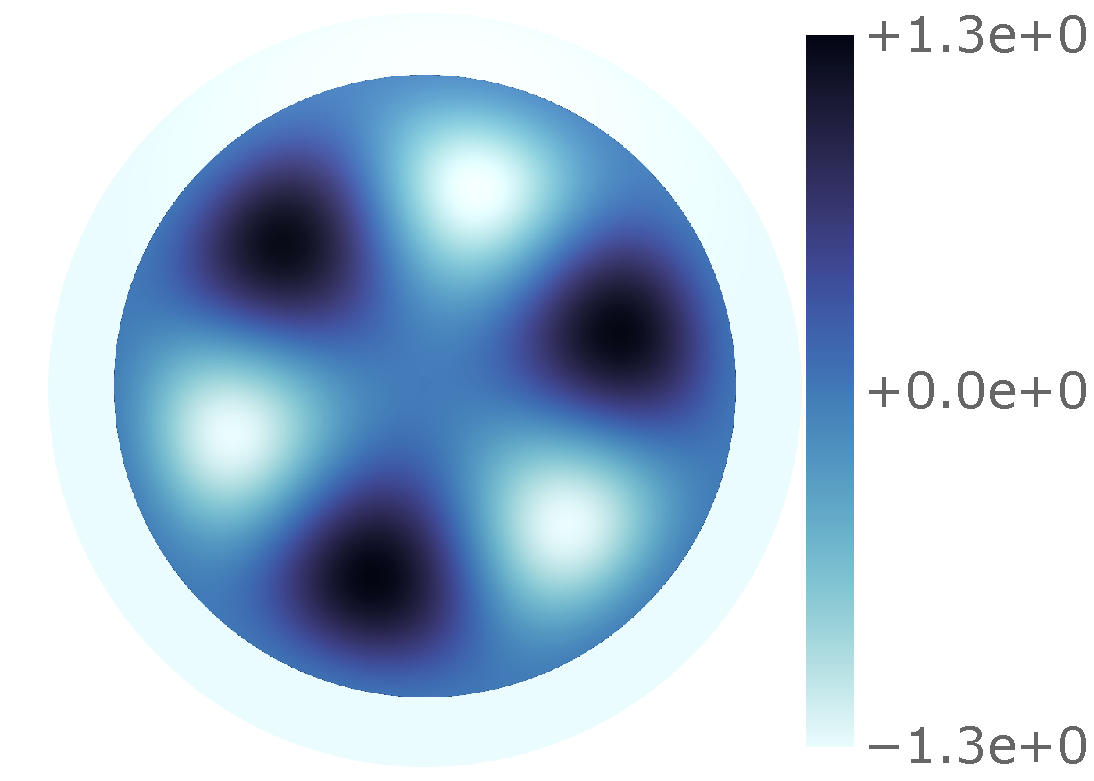
\includegraphics[trim={23 7 3 6},clip,width=.25\textwidth]{slepian_polar40_m-3_rank6_lam9-995528e-01_L16_res128_real.pdf}} % chktex 8
	\hfill
	\subfloat[\(\mu_{8}=0.999553\)]
	{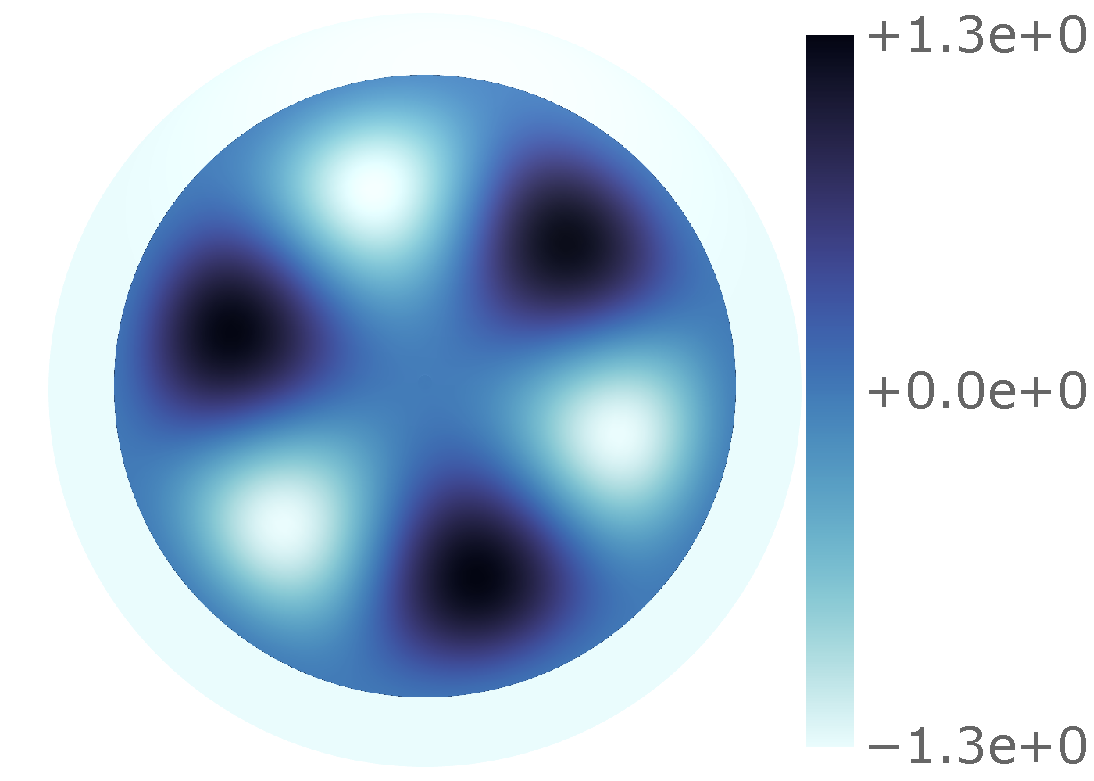
\includegraphics[trim={23 7 3 6},clip,width=.25\textwidth]{slepian_polar40_m3_rank7_lam9-995528e-01_L16_res128_real.pdf}} % chktex 8
	\newline
	\subfloat[\(\mu_{9}=0.998918\)]
	{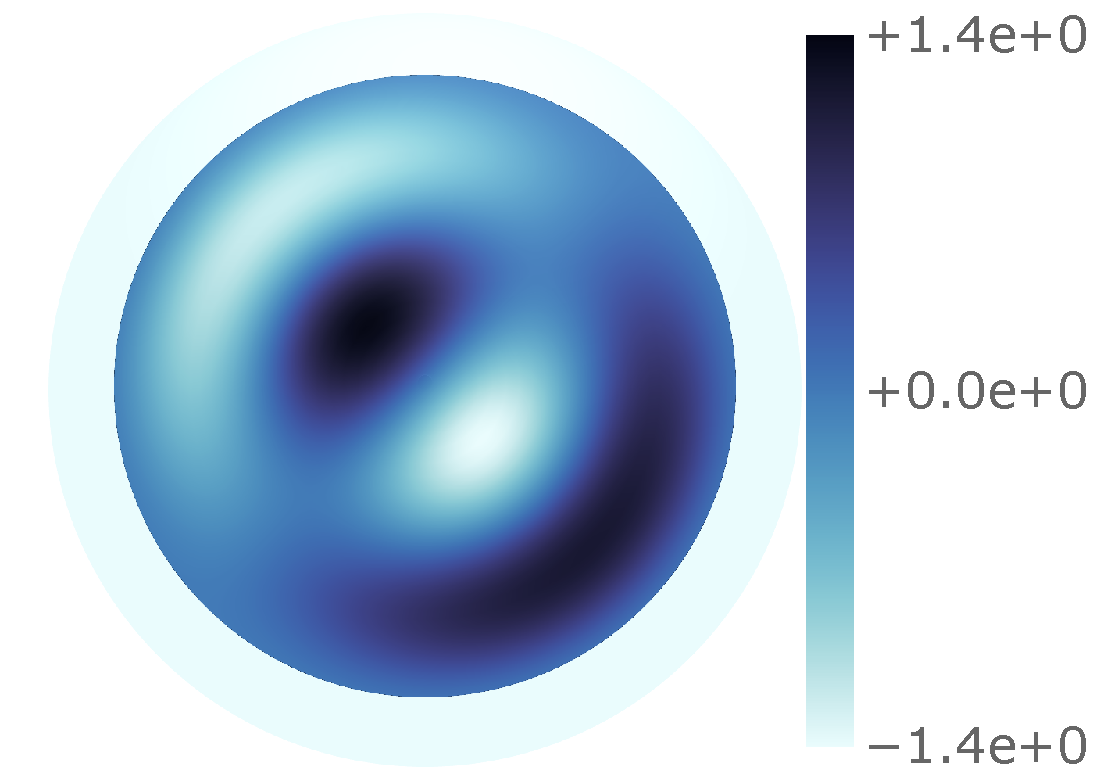
\includegraphics[trim={23 7 3 6},clip,width=.25\textwidth]{slepian_polar40_m-1_rank8_lam9-989180e-01_L16_res128_real.pdf}} % chktex 8
	\hfill
	\subfloat[\(\mu_{10}=0.998918\)]
	{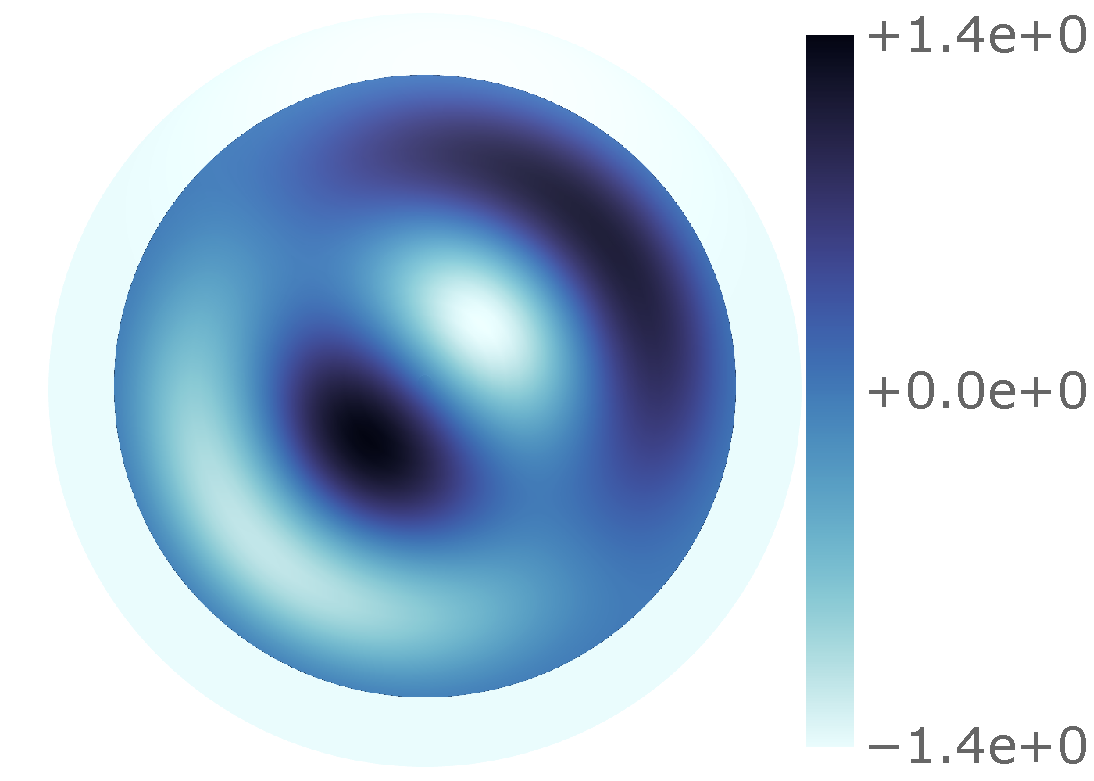
\includegraphics[trim={23 7 3 6},clip,width=.25\textwidth]{slepian_polar40_m1_rank9_lam9-989180e-01_L16_res128_real.pdf}} % chktex 8
	\hfill
	\subfloat[\(\mu_{11}=0.995897\)]
	{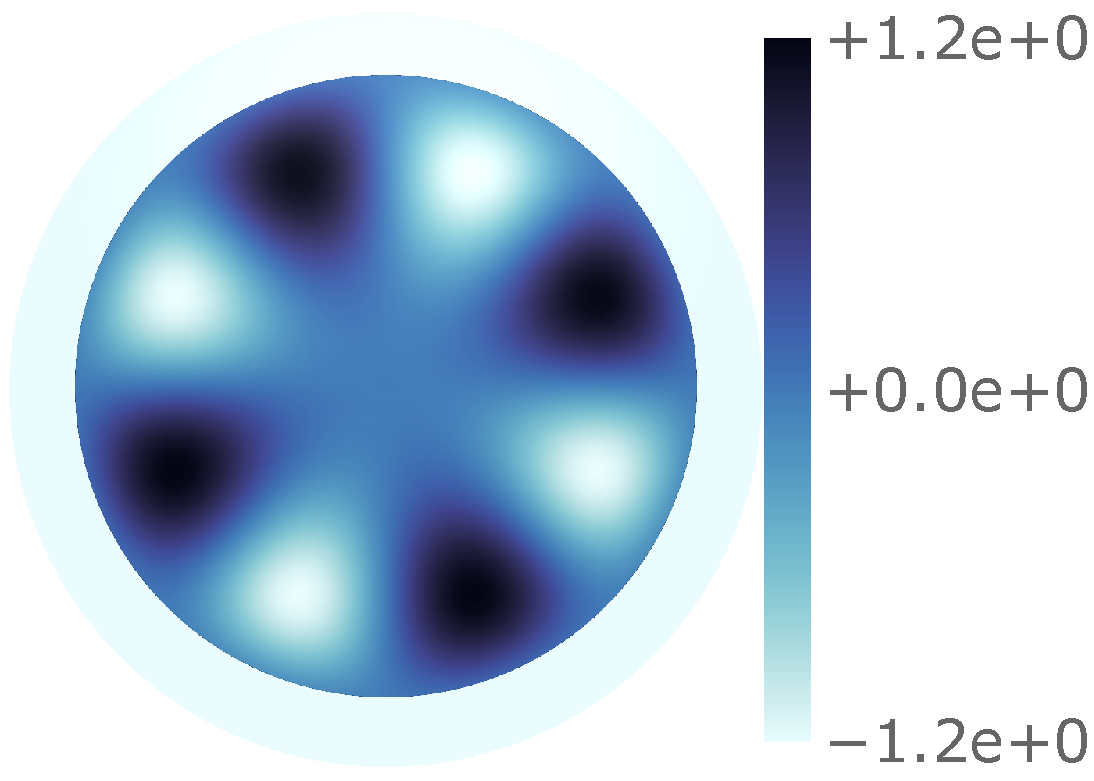
\includegraphics[trim={23 7 3 6},clip,width=.25\textwidth]{slepian_polar40_m-4_rank10_lam9-958971e-01_L16_res128_real.pdf}} % chktex 8
	\hfill
	\subfloat[\(\mu_{12}=0.995897\)]
	{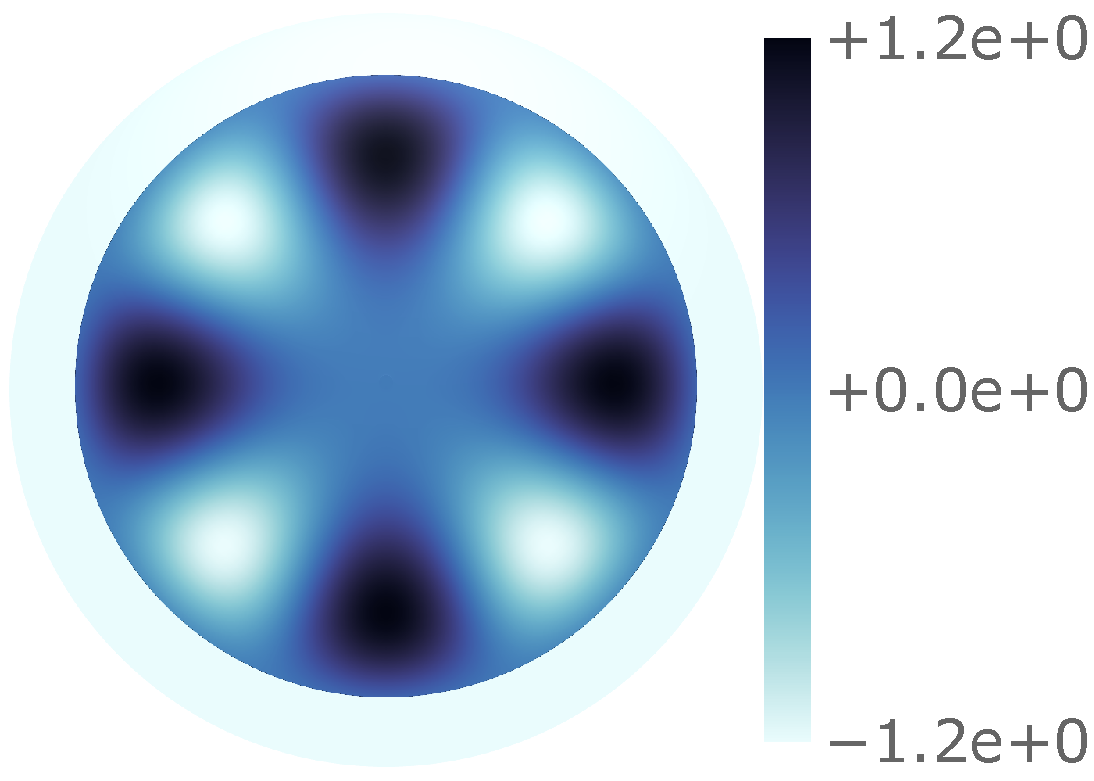
\includegraphics[trim={23 7 3 6},clip,width=.25\textwidth]{slepian_polar40_m4_rank11_lam9-958971e-01_L16_res128_real.pdf}} % chktex 8
	\newline
	\subfloat[\(\mu_{13}=0.988469\)]
	{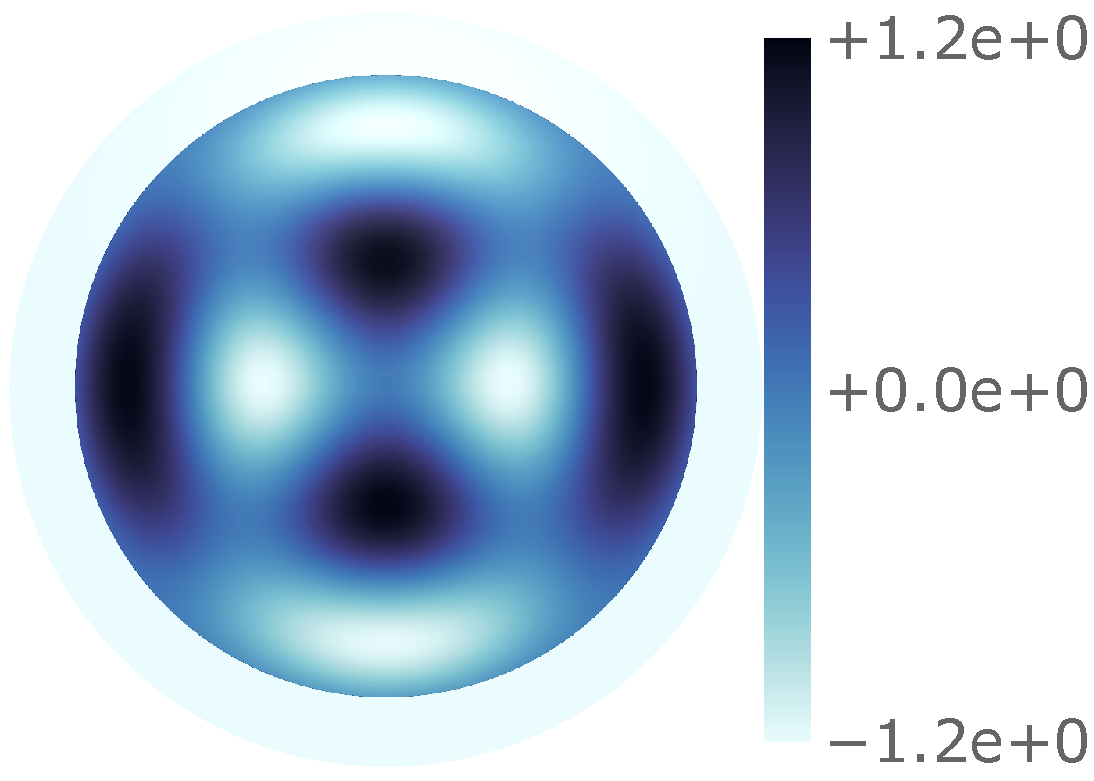
\includegraphics[trim={23 7 3 6},clip,width=.25\textwidth]{slepian_polar40_m-2_rank13_lam9-884688e-01_L16_res128_real.pdf}} % chktex 8
	\hfill
	\subfloat[\(\mu_{14}=0.988469\)]
	{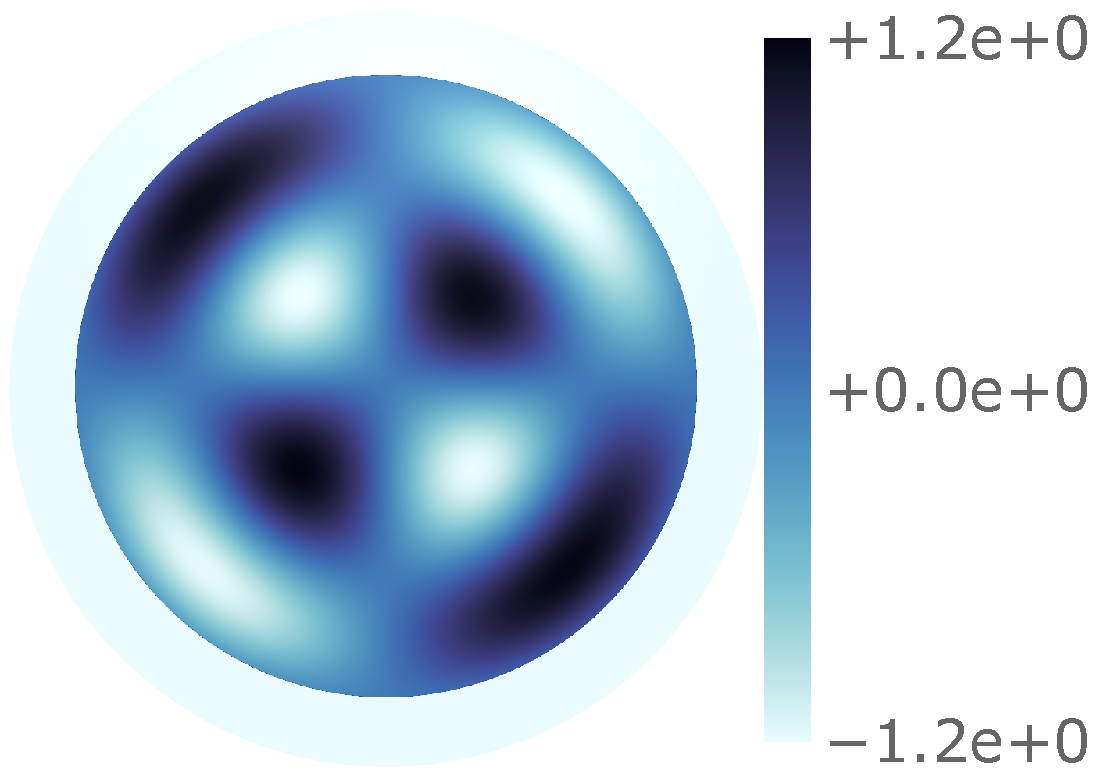
\includegraphics[trim={23 7 3 6},clip,width=.25\textwidth]{slepian_polar40_m2_rank12_lam9-884688e-01_L16_res128_real.pdf}} % chktex 8
	\hfill
	\subfloat[\(\mu_{15}=0.984654\)]
	{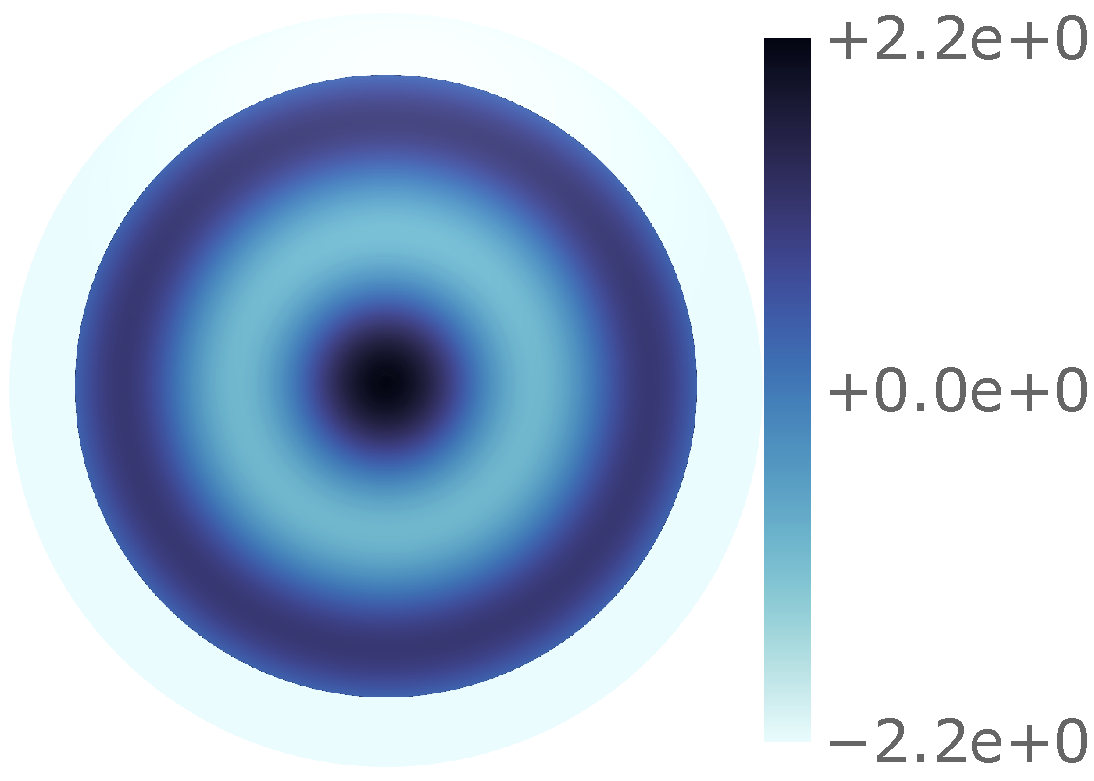
\includegraphics[trim={23 7 3 6},clip,width=.25\textwidth]{slepian_polar40_m0_rank14_lam9-846542e-01_L16_res128_real.pdf}} % chktex 8
	\hfill
	\subfloat[\(\mu_{16}=0.973439\)]
	{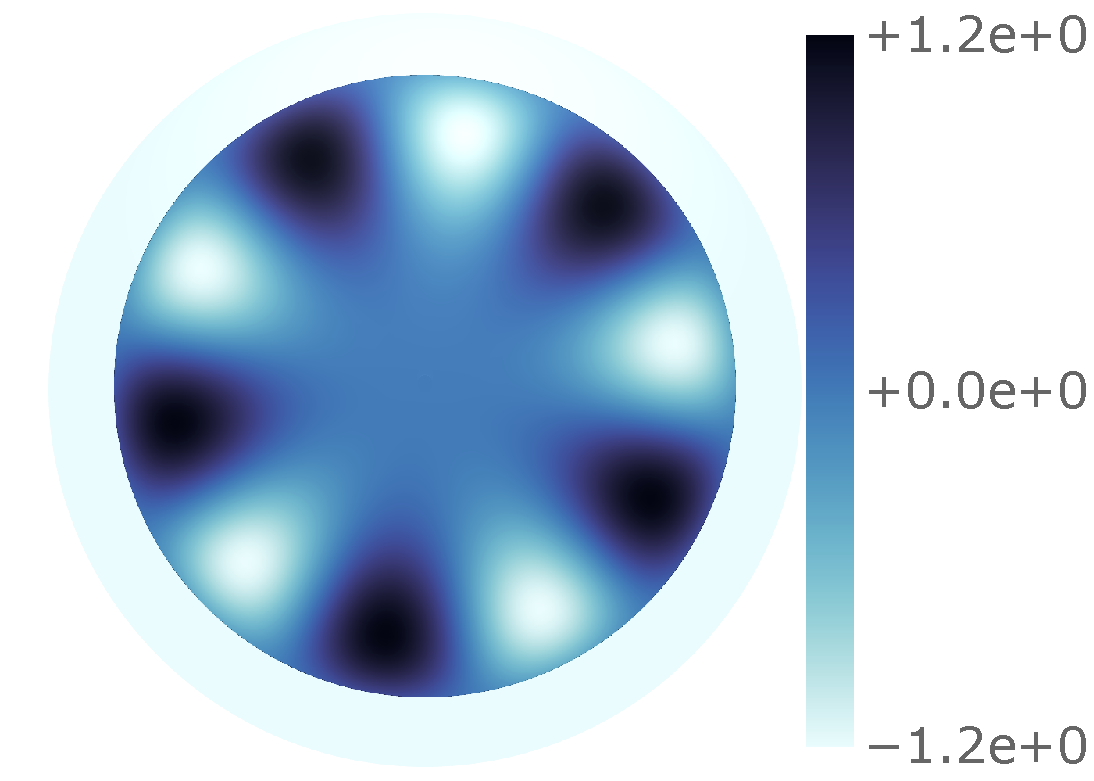
\includegraphics[trim={23 7 3 6},clip,width=.25\textwidth]{slepian_polar40_m5_rank15_lam9-734390e-01_L16_res128_real.pdf}} % chktex 8
	\caption[
		The Slepian functions within a \(\SI{40}{\degree}\) polar cap
	]{
		The first sixteen Slepian functions \(\pixel{\slepian{S}}\) within a polar cap of colatitudinal radius \(\Theta_{0}=\SI{40}{\degree}\).
		The bandlimit here is  \(L=16\), which corresponds to a Shannon number of \(N=30\).
		Ordered by decreasing eigenvalue, the plots are shown left-to-right, top-to-bottom --- indicating worse concentration within the region.
		Note the similarity with the spherical harmonics in this straightforward region.
	}\label{fig:chapter2_slepian_polar_cap}
\end{figure}


\begin{figure}[htpb]
	\centering\capstart{}
	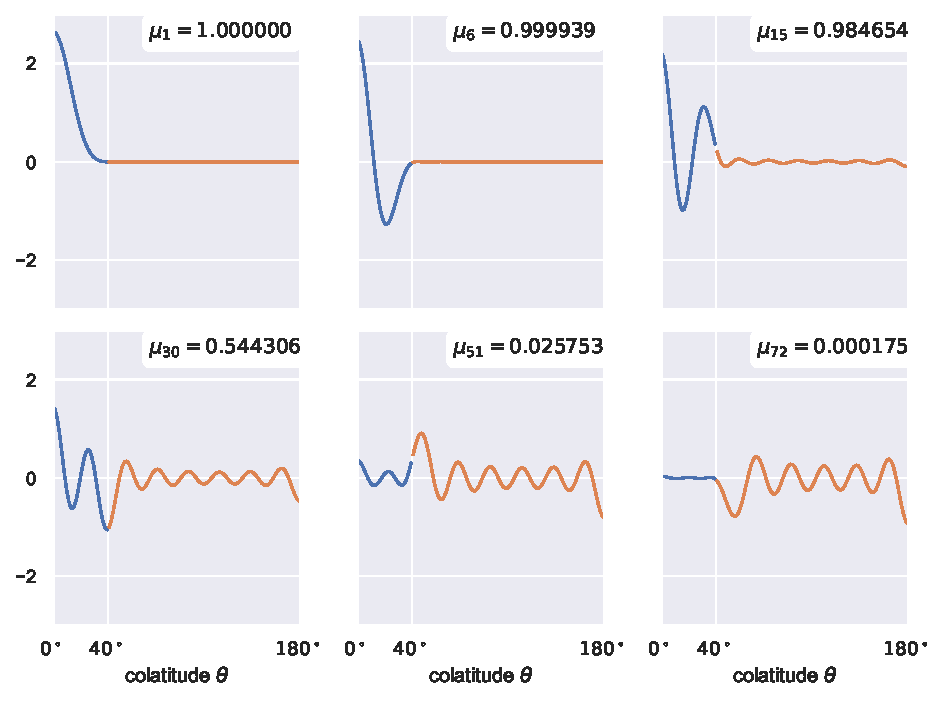
\includegraphics[width=\textwidth]{slepian_colatitude.pdf}
	\caption[
		The colatitudinal dependence of the polar cap Slepian functions
	]{
		The colatitudinal dependence of the Slepian functions \(\pixel{\slepian{S}}\) within a polar cap of colatitudinal radius \(\Theta_{0}=\SI{40}{\degree}\) for \(p \in \set{1, 6, 15, 30, 51, 72}\) shown left-to-right, top-to-bottom.
		The bandlimit here is  \(L=16\), which corresponds to a Shannon number of \(N=30\), \ie{} the final two panels are beyond the Shannon number.
		Blue curves show the concentration within the cap \(\SI{0}{\degree} \leq \theta \leq \Theta_{0}{}\), whilst orange curves show the leakage into the rest of the sphere \(\Theta_{0} < \theta \leq \SI{180}{\degree}\).
		The eigenvalue \(\mu{}\) quantifies the relative spatial concentration of the Slepian function, where lower values have increasing leakage into the orange curve.
	}\label{fig:chapter2_slepian_colatitude}
\end{figure}


\begin{figure}[htpb]
	\centering\capstart{}
	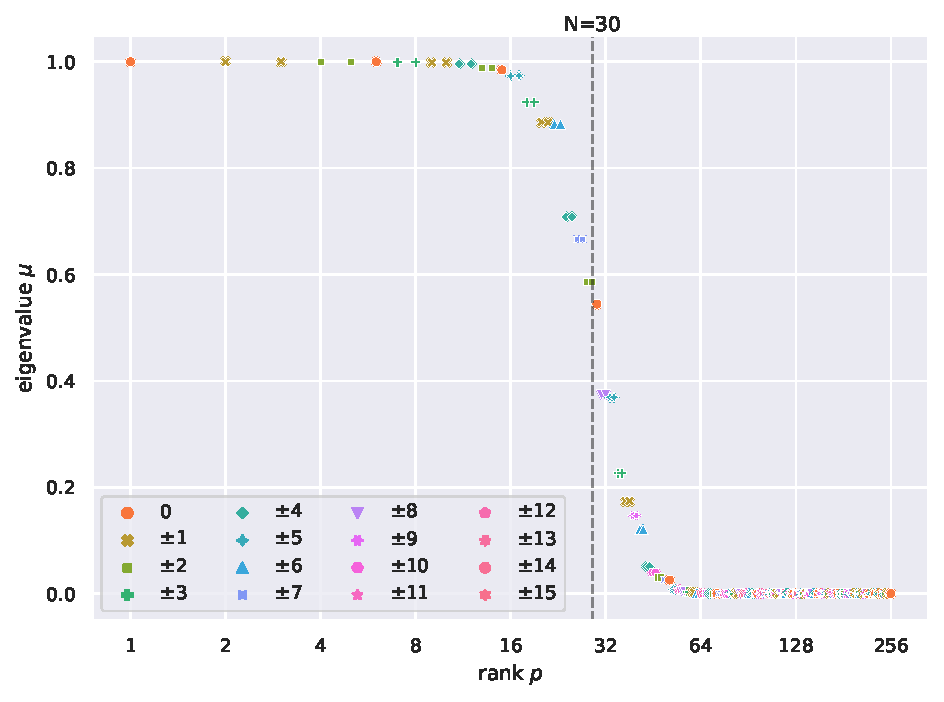
\includegraphics[width=\textwidth]{polar_cap_eigenvalues.pdf}
	\caption[
		The Slepian eigenvalues within a \(\SI{40}{\degree}\) polar cap
	]{
		The ordered Slepian eigenvalues within a polar cap of colatitudinal radius \(\theta_{0}=\SI{40}{\degree}\).
		The bandlimit here is \(L=16\), which corresponds to a Shannon number of \(N=30\), as indicated on the plot.
		Initially, the eigenvalues are \(\almost{1}\), before decreasing rapidly around the Shannon number, and where the majority of the later eigenvalues are \(\almost{0}\).
	}\label{fig:chapter2_polar_cap_eigenvalues}
\end{figure}


\section{Motivation}\label{sec:chapter2_motivation}

As discussed in \cref{sec:chapter2_signals_sphere}, many fields of science and engineering measure data on the sphere.
Often these data are not observed over the whole sphere and are missing in some region.
The polar cap region analysed in \cref{sec:chapter2_spatial_concentration_bandlimited_function} occurs in geodesy, where satellites map out gravitational or magnetic fields of planets whilst flying on inclined polar orbits --- leaving behind a gap between two antipodal axisymmetric polar caps~\cite{Simons2006a}.
In astronomy, ground-based measurements are often confined to a small patches of the sky~\cite{Peebles1973,Tegmark1995}.
Groundtruthing is not typically possible in planetary science, and as such, knowledge of estimation statistics of properties observed over portions of the planetary surface is imperative.
In geomagnetism, one is interested in the field value over the whole of the Earth's surface, but in practice can only make a finite number of measurements.
Lastly, in cosmology, the sky is effectively a sphere observed from inside out, and observations of the cosmic microwave background are masked by the Galactic plane~\cite{Tegmark1996,Hinshaw2003}.
Cosmology has been the primary motivating factor of this thesis, and as such, \cref{sec:chapter2_cosmic_microwave_background} follows with more detail on the cosmic microwave background.

\subsection{Cosmic Microwave Background (CMB)}\label{sec:chapter2_cosmic_microwave_background}

In the early Universe, the temperature was sufficiently hot such that photons had enough energy to ionise neutral hydrogen.
Photons were tightly coupled to electrons through Compton scattering, which in turn were coupled to baryons through electromagnetic interactions.
The mean free path of photons was tiny due to frequent scattering.
Thus, the Universe at this point consisted of an opaque photon-baryon fluid.
Over time, this primordial plasma cooled as the Universe expanded until photons were no longer sufficiently energetic to ionise neutral hydrogen.
As a result, the fraction of ionised electrons decreased, the photons decoupled from the baryons, and the Universe became effectively transparent to radiation.
This process occurred when the temperature of the Universe fell to \(\almost{\SI{3000}{\kelvin}}\), corresponding to a redshift \(z_{\text{rec}} \almost{1000}\), and is known as recombination.
The surface of last scattering refers to the end of recombination, which is when the photons last scattered.
The CMB radiation observed today is from these photons, which were free to propagate (largely) unobstructed through space.

Before recombination, the Universe was in thermal equilibrium and exhibited a blackbody spectrum.
This thermal spectrum is still present now, despite the redshifting of photons as they propagated through the expanding Universe.
CMB photons are observed today as a near-perfect blackbody spectrum in the microwave frequency range, with a mean temperature of \(\mean{T} = \SI{2.72548(0.00057)}{\kelvin}\)~\cite{Fixsen2009}.
Moreover, the CMB spectrum is the most precisely measured blackbody spectrum in nature~\cite{White1994}.
The CMB is highly isotropic --- primordial perturbations generate anisotropies in the CMB at a level of just \(10^{-5}\).
However, the dipole contribution in the CMB is not considered in cosmological analyses, as this is not of cosmological origin.
The anisotropies induced in the CMB dipole (at a level of \(10^{-3}\)) occur due to the Doppler shift created by the relative motion between the Solar System and the CMB rest frame.
It is the small anisotropies that contain the majority of the cosmological information.
For more detail on the physics of the anisotropies of the CMB see~\cite{Bucher2015}.

\cref{fig:chapter2_planck_frequency} presents maps of the fluctuations of sky emission in each of the nine Planck frequency bands, upon removal of a common dipole moment.
Note that at all frequencies \(\qtylist[list-units=single]{30;44;70;100;143;217;353;545;857}{\giga\hertz}\), the CMB is obstructed by foreground microwave emissions from the Galactic bulge.
In cosmology, one observes the projection of some three-dimensional random field onto the celestial sphere.
For example, the CMB anisotropies are mainly the projection of photon density, bulk velocity, and gravitational potential over the surface of last scattering.
The language used to describe random fields on the sphere is now described in \cref{sec:chapter2_statistics_random_fields_sphere}.

\begin{figure}[htpb]
	\centering\capstart{}
	\includegraphics[trim={0 200 0 0},clip,width=\textwidth]{planck_2018_temp_freq.pdf}
	\includegraphics[trim={1100 0 1100 2100},clip,width=\textwidth]{planck_2018_temp_freq.pdf}
	\caption[
		The 2018 \emph{Planck} maps in intensity in each frequency band
	]{
		Fluctuations of sky emission in each of nine \emph{Planck} frequency bands, after removal of a common dipole component (courtesy of \emph{The Planck Collaboration 2018}~\cite{Planck2020}).
		Note that the CMB is obstructed by the foreground microwave emissions of the Milky Way at all frequencies.
	}\label{fig:chapter2_planck_frequency}
\end{figure}


\subsection{Statistics of Random Fields on the Sphere}\label{sec:chapter2_statistics_random_fields_sphere}

The current favoured model for creating fluctuations in the Universe is cosmological inflation.
Due to the quantum nature of inflation, one cannot predict the exact shape of the Universe, but only its statistical properties.
Many realisations of the Universe are statistically equivalent.
To compare theory and observation, one must measure statistical properties of the Universe, and compare these to the same statistical properties evaluated on a model of the Universe.
The cosmological principle states that, on sufficiently large scales, the Universe is invariant under rotations (statistically isotropic) and invariant under translations (statistically homogeneous).
Here, only zero-mean fields are considered, such as the temperature fluctuations in the CMB or the matter overdensity.

\subsubsection{Power Spectrum}

Consider a three-dimensional, zero-mean, random field \(f(\vb*{x})\).
The probability of realising some field configuration is a functional.
Correlators of fields are expectation values of products of fields at different spatial points.
In Fourier space, the two-point correlator (or power spectrum) is given by
%
\begin{equation}\label{eq:chapter2_power_spectrum}
	\expval*{\fourier{f}(\vb*{k}) \conj{\fourier{f}}(\vb*{k'})}
	%
	= {(2\pi)}^{3} \delta^{3}(\vb*{k} - \vb*{k'}) \powerSpectrumDim{f},
\end{equation}
%
where \(\powerSpectrumDim{f}\) is the dimensionless power spectrum which, by statistical isotropy, depends only on the magnitude of \(k=\abs{\vb*{k}}\).
Due to statistical homogeneity, the Dirac delta function is present in \cref{eq:chapter2_power_spectrum}, such that the correlator is invariant under spatial translations.
Often one considers the power in a shell, rather than per unit Fourier space volume, \ie{}
%
\begin{equation}\label{eq:chapter2_power_shell}
	\powerSpectrumShell{f}
	%
	= \frac{k^{3}\powerSpectrumDim{f}}{2\pi^{2}},
\end{equation}
%
such that
%
\begin{equation}
	\powerSpectrumShell{f} \dd{\ln{k}}
	%
	= \frac{\dd[3]{\vb*{k}}}{{(2\pi)}^{3}} \powerSpectrumDim{f},
\end{equation}
%
after integrating out the angular part.
The Fourier convention adopted here is
%
\begin{equation}
	f(\vb*{x})
	%
	= \int\frac{\dd[3]{\vb*{k}}}{{(2\pi)}^{3}} \fourier{f}(\vb*{k}) \exp(i\vb*{k}\cdot\vb*{x})
\end{equation}
%
(\cf{} \cref{eq:chapter2_fourier_time}), and
%
\begin{equation}
	\fourier{f}(\vb*{k})
	%
	= \int\dd[3]{\vb*{x}} f(\vb*{x}) \exp(-i\vb*{k}\cdot\vb*{x})
\end{equation}
%
(\cf{} \cref{eq:chapter2_fourier_frequency}).
Note for real fields, the following conjugate symmetry relation holds
%
\begin{equation}
	\fourier{f}(\vb*{k})
	%
	= \conj{\fourier{f}}(-\vb*{k}),
\end{equation}
%
and similarly
%
\begin{equation}
	f(\vb*{x})
	%
	= \conj{f}(-\vb*{x}).
\end{equation}

For linearly evolved fluctuations from single field inflation, the power spectrum is sufficient to describe the statistics.
However, sometimes higher order statistics are required to analyse deviations from straightforward inflationary models.
The simplest of these is the three-point correlator
%
\begin{equation}
	\expval*{f(\vb*{k}_{1}) f(\vb*{k}_{2}) f(\vb*{k}_{3})}
	%
	= {(2\pi)}^{3} \delta^{3}(\vb*{k}_{1} + \vb*{k}_{2} + \vb*{k}_{3}) \bispectrum{f},
\end{equation}
%
which gives rise to the bispectrum \(\bispectrum{f}\) which is a symmetric function (due to statistical isotropy) of the three wavenumbers.
The Dirac delta again appears due to statistical homogeneity.
Although starting with nine degrees of freedom (due to the three three-dimensional wavevectors), the bispectrum only depends on three of these.
Statistical isotropy and homogeneity both remove three of these degrees of freedom.
The three-point correlator depends solely on the three rotational-invariants associated with the triangular configurations of the three wavevectors --- which are the magnitudes.
The three-point correlator vanishes for zero-mean Gaussian random fields, and as such provides a good test of theories, \ie{} straightforward inflationary models which predict near-Gaussian primordial perturbations.
Other higher order statistics may be computed, such as the four-point correlator
%
\begin{align}
	\expval*{f(\vb*{k}_{1}) f(\vb*{k}_{2}) f(\vb*{k}_{3}) f(\vb*{k}_{4})} =
	%
	\begin{aligned}
		 & {(2\pi)}^{3} \delta^{3}(\vb*{k}_{1} + \vb*{k}_{2} + \vb*{k}_{3} + \vb*{k}_{4}) \\
		%
		 & \times \trispectrum{f},
	\end{aligned}
\end{align}
%
where the trispectrum \(\trispectrum{f}\) here depends on just six degrees of freedom (down from an initial twelve).

\subsubsection{Rotations of Random Fields}

The two-point function must be invariant under all rotations due to statistical isotropy, which implies
%
\begin{equation}
	\expval*{\harmonic{f} \conj{\harmonic[']{f}}}
	%
	= \expval*{\harmonic{(\rotation{\rho}f)}\harmonic[']{(\rotation{\rho}f)}}.
\end{equation}
%
This only holds if
%
\begin{equation}
	\expval*{\harmonic{f} \conj{\harmonic[']{f}}}
	%
	= \powerSpectrum \delta_{\ell\ell'} \delta_{m m'},
\end{equation}
%
as
%
\begin{align}
	\expval*{\harmonic{f} \conj{\harmonic[']{f}}}
	%
	 & = \expval*{\harmonic{(\rotation{\rho}f)}\harmonic[']{(\rotation{\rho}f)}} \nonumber{}                                                                \\
	%
	 & = \wignerSum \wignerSum['] \wigner{\ell}{m}{n}(\rho) \wigner[\ast]{\ell'}{m'}{n'}(\rho) \expval*{f_{\ell n} \conj{f_{\ell' n'}}} \nonumber{}         \\
	%
	 & = \wignerSum \wignerSum['] \wigner{\ell}{m}{n}(\rho) \wigner[\ast]{\ell'}{m'}{n'}(\rho) \powerSpectrum \delta_{\ell \ell'} \delta_{n n'} \nonumber{} \\
	%
	 & = \powerSpectrum \delta_{\ell\ell'} \wignerSum \wigner{\ell}{m}{n}(\rho) \wigner[\ast]{\ell'}{m'}{n}(\rho) \nonumber{}                               \\
	%
	 & = \powerSpectrum \delta_{\ell\ell'} \delta_{m m'}.
\end{align}
%
The real quantity \(\powerSpectrum{}\) is the angular power spectrum of \(\pixel{f}\).
Zero-mean Gaussian random fields are fully determined by their two-point function and hence their power spectrum.
In real space the two-point function is
%
\begin{align}
	\expval*{f(\omega) \conj{f}(\omega')}
	%
	 & = \sum\limits_{\ell=0}^{\infty} \sum\limits_{m=-\ell}^{\ell} \sum\limits_{\ell'=0}^{\infty} \sum\limits_{m'=-\ell'}^{\ell'} \expval*{\harmonic{f} \conj{\harmonic[']{f}}} \harmonic{Y}(\omega) \conj{\harmonic[']{Y}}(\omega') \nonumber{}   \\
	%
	 & = \sum\limits_{\ell=0}^{\infty} \sum\limits_{m=-\ell}^{\ell} \sum\limits_{\ell'=0}^{\infty} \sum\limits_{m'=-\ell'}^{\ell'} \powerSpectrum \delta_{\ell\ell'} \delta_{m m'} \harmonic{Y}(\omega) \conj{\harmonic[']{Y}}(\omega') \nonumber{} \\
	%
	 & = \sum\limits_{\ell=0}^{\infty} \powerSpectrum \sum\limits_{m=-\ell}^{\ell} \harmonic{Y}(\omega) \conj{\harmonic{Y}}(\omega') \nonumber{}                                                                                                    \\
	%
	 & = \sum\limits_{\ell=0}^{\infty} \factor \powerSpectrum P_{\ell}(\omega\cdot\omega')  \nonumber{}                                                                                                                                             \\
	%
	 & = C(\theta),
\end{align}
%
where the penultimate line follows by the spherical harmonic addition theorem \cref{eq:chapter2_addition_theorem}, and in the last line \({\omega\cdot\omega' = \cos{\theta}}\).
Hence, the two-point function depends on the angle between the two points, as required by statistical isotropy.
The variance of the field is
%
\begin{equation}
	C(0)
	%
	= \sum\limits_{\ell=0}^{\infty} \factor \powerSpectrum
	%
	\approx \int\dd{\ln{\ell}} \frac{\ell(\ell+1) \powerSpectrum}{2\pi}.
\end{equation}
%
Inverting the correlation function retrieves the power spectrum using the orthogonality of the Legendre polynomials
%
\begin{equation}
	\powerSpectrum
	%
	= 2\pi \int\limits_{-1}^{1} \dd{\cos{\theta}} \pixel{C} P_{\ell}(\cos{\theta}).
\end{equation}

\subsubsection{Projection of Three-Dimensional Random Fields}

The CMB decoupled from matter around recombination.
The temperature anisotropies observed are the projection of the conditions at that time over the surface of last scattering.
A statistically isotropic two-dimensional field on the sphere is the projection of a three-dimensional statistically isotropic and homogeneous random field.
Consider projecting a random field \(F(\vb*{x})\) (for example, CMB temperature fluctuations) over a sphere of radius \(r\) (the distance to the surface of last scattering), centred on the origin, \ie{}
%
\begin{equation}
	f(\vu*{n})
	%
	= F(r\vu*{n}),
\end{equation}
%
where \(\vu*{n}\) is a unit vector along the line-of-sight.
Consider the expansion of \(F(r\vu*{n})\) in Fourier space
%
\begin{equation}
	f(\vu*{n})
	%
	= F(r\vu*{n})
	%
	= \int\frac{\dd[3]{\vb*{k}}}{{(2\pi)}^{3}} \fourier{F}(\vb*{k}) \exp(i k r\vu*{k}\cdot\vu*{n}),
\end{equation}
%
and the Rayleigh plane-wave expansion
%
\begin{align}
	\exp(i k r\vu*{k}\cdot\vu*{n})
	%
	 & = \sum\limits_{\ell=0}^{\infty} (2\ell+1) i^{\ell} \bessel{k r} P_{\ell}(\vu*{k}\cdot\vu*{n}) \nonumber{}                                   \\
	%
	 & = 4\pi \sum\limits_{\ell=0}^{\infty} i^{\ell} \bessel{k r} \sum\limits_{m=-\ell}^{\ell} \conj{\harmonic{Y}}(\vu*{k}) \harmonic{Y}(\vu*{n}),
\end{align}
%
where \(\bessel{k r}\) are the spherical Bessel functions.
The spherical harmonic coefficients of \(f(\vu*{n})\) are therefore
%
\begin{align}
	\harmonic{f}
	%
	 & = \integrateSphere{\vu*{n}} f(\vu*{n}) \conj{\harmonic{Y}}(\vu*{n}) \nonumber{}                                                                                                                                                                                                                       \\
	%
	 & = \integrateSphere{\vu*{n}} \bigg[\int\frac{\dd[3]{\vb*{k}}}{{(2\pi)}^{3}} \fourier{F}(\vb*{k}) \exp(i k r\vu*{k}\cdot\vu*{n})\bigg] \conj{\harmonic{Y}}(\vu*{n}) \nonumber{}                                                                                                                         \\
	%
	 & = \int\frac{\dd[3]{\vb*{k}}}{{(2\pi)}^{3}} \fourier{F}(\vb*{k}) \integrateSphere{\vu*{n}} \bigg[4\pi \sum\limits_{\ell'=0}^{\infty} i^{\ell'} \bessel[']{k r} \sum\limits_{m'=-\ell'}^{\ell'} \conj{\harmonic[']{Y}}(\vu*{k}) \harmonic[']{Y}(\vu*{n})\bigg] \conj{\harmonic{Y}}(\vu*{n}) \nonumber{} \\
	%
	 & = 4\pi i^{\ell} \int\frac{\dd[3]{\vb*{k}}}{{(2\pi)}^{3}} \fourier{F}(\vb*{k}) \bessel{k r} \conj{\harmonic{Y}}(\vu*{k}) \nonumber{}                                                                                                                                                                   \\
	%
	 & = i^{\ell} \int\frac{\dd[3]{\vb*{k}}}{2\pi^{2}} \fourier{F}(\vb*{k}) \bessel{k r} \conj{\harmonic{Y}}(\vu*{k}),
\end{align}
%
where the penultimate line follows by the orthonormality of the spherical harmonics \cref{eq:chapter2_spherical_harmonics_orthonormal}.
The two-point function in harmonic space is hence
%
\begin{align}
	\expval*{\harmonic{f}\conj{\harmonic[']{f}}}
	%
	 & = i^{\ell-\ell'} \int\frac{\dd[3]{\vb*{k}}}{2\pi^{2}} \int\frac{\dd[3]{\vb*{k'}}}{2\pi^{2}} \expval*{\fourier{F}(\vb*{k}) \conj{\fourier{F}}(\vb*{k'})} \bessel{k r} \bessel[']{k'r} \conj{\harmonic{Y}}(\vu*{k}) \harmonic[']{Y}(\vu*{k'}) \nonumber{} \\
	%
	 & = \frac{i^{\ell-\ell'}}{\pi/2} \int\dd[3]{\vb*{k}} \int\dd[3]{\vb*{k'}} [\delta^{3}(\vb*{k} - \vb*{k'}) \powerSpectrumDim{f}] \bessel{k r} \bessel[']{k'r} \conj{\harmonic{Y}}(\vu*{k}) \harmonic[']{Y}(\vu*{k'}) \nonumber{}                           \\
	%
	 & = \frac{i^{\ell-\ell'}}{\pi/2} \int\dd[3]{\vb*{k}} \powerSpectrumDim{f} \bessel{k r} \bessel[']{k r} \conj{\harmonic{Y}}(\vu*{k}) \harmonic[']{Y}(\vu*{k}) \nonumber{}                                                                                  \\
	%
	 & = \frac{i^{\ell-\ell'}}{\pi/2} \bigg[\int\dd{k} k^{2} \integrateSphere{\vu*{k}}\bigg] \powerSpectrumDim{f} \bessel{k r} \bessel[']{k r} \conj{\harmonic{Y}}(\vu*{k}) \harmonic[']{Y}(\vu*{k}) \nonumber{}                                               \\
	%
	 & = 4\pi i^{\ell-\ell'} \int\frac{\dd{k}}{k} \frac{k^{3}\powerSpectrumDim{f}}{2\pi^{2}} \bessel{k r} \bessel[']{k r} \integrateSphere{\vu*{k}} \conj{\harmonic{Y}}(\vu*{k}) \harmonic[']{Y}(\vu*{k}) \nonumber{}                                          \\
	%
	 & = 4\pi \delta_{\ell\ell'} \delta_{m m'} \int\dd{\ln{k}} \Delta_{f}^{2}(k) j^{2}_{\ell}(k r) \nonumber{}                                                                                                                                                 \\
	%
	 & = \powerSpectrum \delta_{\ell\ell'} \delta_{m m'},
\end{align}
%
where the penultimate line follows by \cref{eq:chapter2_power_shell}.
Thus, \(f(\vu*{n})\) is a statistically isotropic field with angular power spectrum
%
\begin{equation}
	\powerSpectrum
	%
	= 4\pi \int\dd{\ln{k}} \Delta_{f}^{2}(k) j^{2}_{\ell}(k r).
\end{equation}

\subsubsection{Cosmic Variance}

It is impossible to predict the exact form that cosmological fields must take.
A given model makes a prediction for the probability distribution, from which one draws the single realisation of the fields observed.
An estimate made of the properties of the underlying probability distribution, \ie{} its power spectrum, has some random error due to attempting to estimate ensemble-averaged quantities from a single realisation.
Cosmic variance is the random error which contributes to the error budget of most inferences made in observational cosmology.
Whilst this is not the dominant error if the measurements are noisy, cosmologists aim to reach this cosmic variance limit.
Consider estimating the angular power spectrum of a zero-mean random field \(f(\omega)\), supposing that the observations that existed are full-sky and noise-free.
The estimator for the \(\powerSpectrum{}\) is as follows
%
\begin{equation}
	\powerSpectrumHat
	%
	= \frac{1}{2\ell+1} \sum\limits_{m=-\ell}^{\ell} \harmonic{f} \conj{\harmonic{f}}.
\end{equation}
%
This estimator is unbiased, \ie{} \(\expval*{\powerSpectrumHat} = \powerSpectrum{}\), as
%
\begin{align}
	\expval*{\powerSpectrumHat}
	%
	 & = \frac{1}{2\ell+1} \sum\limits_{m=-\ell}^{\ell} \expval*{\harmonic{f} \conj{\harmonic{f}}} \nonumber{} \\
	%
	 & = \frac{1}{2\ell+1} \sum\limits_{m=-\ell}^{\ell} \powerSpectrum \nonumber{}                             \\
	%
	 & = \powerSpectrum.
\end{align}
%
Here, the sum in \(m\) means for a given \(\ell{}\) one uses all the available information in the \(2\ell+1\) independent degrees of freedom; however, this estimator has non-zero variance.
The variance of a Gaussian random field follows by
%
\begin{align}
	\variance{\powerSpectrumHat}
	%
	 & = - \expval*{\powerSpectrumHat}^{2} + \expval*{\powerSpectrumHat^{2}} \nonumber{}                                                                                                                     \\
	%
	 & = - \powerSpectrum^{2} + \frac{1}{{(2\ell+1)}^{2}} \sum\limits_{m=-\ell}^{\ell} \sum\limits_{m'=-\ell'}^{\ell'} \expval*{\harmonic{f} \conj{\harmonic{f}} f_{\ell m'} \conj{f_{\ell m'}}} \nonumber{} \\
	%
	 & = - \powerSpectrum^{2} + \frac{1}{{(2\ell+1)}^{2}} \sum\limits_{m=-\ell}^{\ell} \sum\limits_{m'=-\ell'}^{\ell'}
	%
	\begin{aligned}
		 & \expval*{\harmonic{f} \conj{\harmonic{f}}}  \expval*{f_{\ell m'} \conj{f_{\ell m'}}} \nonumber{}  \\
		%
		 & + \expval*{\harmonic{f} f_{\ell m'}} \expval*{\conj{\harmonic{f}} \conj{f_{\ell m'}}} \nonumber{} \\
		%
		 & + \expval*{\harmonic{f} \conj{f_{\ell m'}}} \expval*{\conj{\harmonic{f}} f_{\ell m'}}
	\end{aligned} \nonumber{}                                          \\
	%
	 & = \frac{1}{{(2\ell+1)}^{2}} \sum\limits_{m=-\ell}^{\ell} \sum\limits_{m'=-\ell'}^{\ell'}
	%
	\begin{aligned}
		 & \expval*{\harmonic{f} f_{\ell m'}} \expval*{\conj{\harmonic{f}} \conj{f_{\ell m'}}} \nonumber{} \\
		%
		 & + \expval*{\harmonic{f} \conj{f_{\ell m'}}} \expval*{\conj{\harmonic{f}} f_{\ell m'}}
	\end{aligned} \nonumber{}                                                                \\
	%
	 & = \frac{1}{{(2\ell+1)}^{2}} \sum\limits_{m=-\ell}^{\ell} \sum\limits_{m'=-\ell'}^{\ell'}
	%
	\begin{aligned}
		 & \phaseFactor['] \expval*{\harmonic{f} \conj{f_{\ell(-m')}}} \phaseFactor['] \expval*{\conj{\harmonic{f}} f_{\ell(-m')}} \nonumber{} \\
		%
		 & + \powerSpectrum^{2} \delta_{m m'}
	\end{aligned} \nonumber{}                                \\
	%
	%
	 & = \frac{2}{{(2\ell+1)}^{2}} \sum\limits_{m=-\ell}^{\ell} \powerSpectrum^{2} \nonumber{}                                                                                                               \\
	%
	 & = \frac{2}{2\ell+1} \powerSpectrum^{2},
\end{align}
%
where the third line follows by Wick's theorem.
Irreducible cosmic variance arises from having \(2\ell+1\) independent modes at each \(\ell{}\) with which to estimate the variance of their distribution.
Cosmic variance dominates the current measurements of the error bars of the angular power spectrum of the CMB temperature anisotropies at low-\(\ell{}\), as shown in \cref{fig:chapter2_power_spectrum}.

\begin{figure}[htpb]
	\centering\capstart{}
	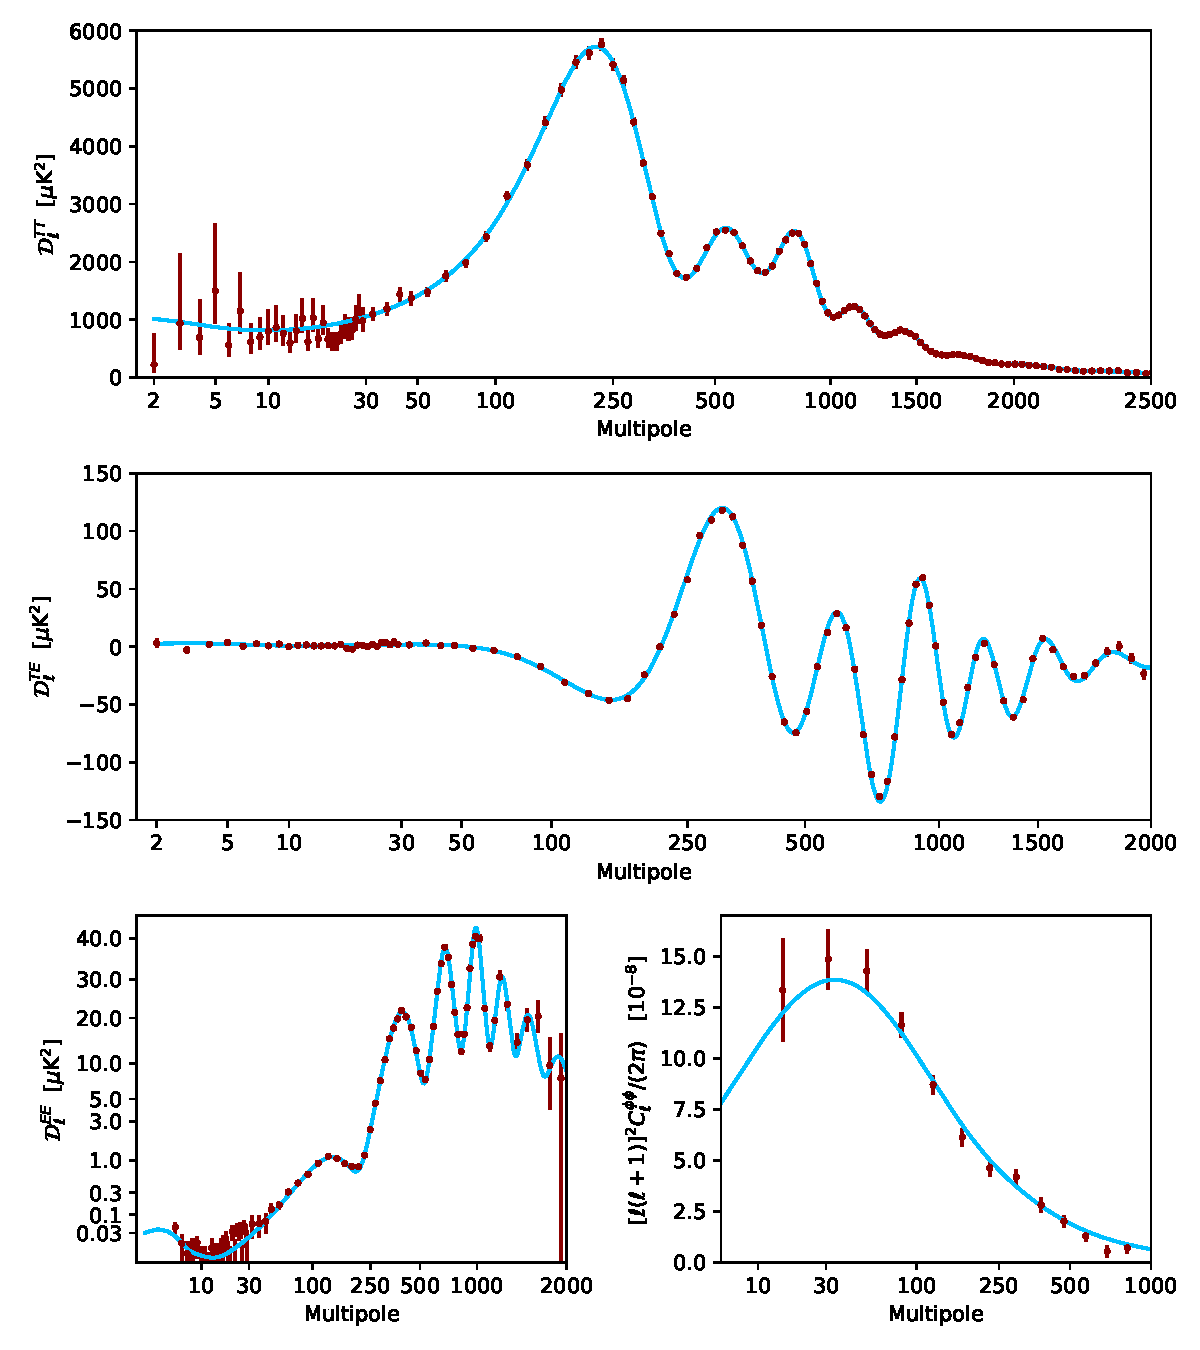
\includegraphics[trim={0 430 0 0},clip,width=\textwidth]{planck_2018_power_spectrum.pdf}
	\caption[
        The 2018 Planck CMB angular power spectrum in temperature
	]{
        Measurements of the angular power spectrum of the Planck CMB temperature anisotropies (in red), where \(D_{\ell}^{TT} = \ell(\ell+1)C_{\ell}/(2\pi)\) (courtesy of The Planck Collaboration 2018~\cite{Planck2020}).
        The blue line is a best-fit model to temperature and polarisation data.
        The error bars at low-\(\ell{}\) are dominated by cosmic variance.
	}\label{fig:chapter2_power_spectrum}
\end{figure}


\section{Outlook}\label{sec:chapter2_outlook}

In practice, the statistical methods used to analyse random fields on the sphere, discussed in \cref{sec:chapter2_statistics_random_fields_sphere}, are not suitable when data are only measured over a partial region.
Therefore, one must either fill in the data by some method (\eg{} interpolation, statistics, machine learning, or simply setting the values to zero) or design methods to work only with the data that are present.
\cref{fig:chapter2_planck_masked} demonstrates this latter case for the Planck temperature map, where the \texttt{Commander}~\cite{Eriksen2004,Eriksen2008,Planck2016} mask is applied (in grey) which blocks out the foreground microwave emissions (which can be seen in \cref{fig:chapter2_planck_frequency}).
In \cref{sec:chapter2_limitations_existing_approaches}, limitations of existing approaches are discussed, in particular signal analysis as well as more general analysis techniques.
The aim of this thesis follows in \cref{sec:chapter2_thesis_aim}.

\begin{figure}[htpb]
\centering\capstart{}
\includegraphics[width=\textwidth]{planck_2018_temp_mask.pdf}
\caption[
The 2018 Planck CMB map with the \texttt{Commander} mask
]{
The Planck \texttt{Commander}~\cite{Eriksen2004,Eriksen2008,Planck2016,Planck2020a} CMB temperature map used in low-\(\ell{}\) temperature likelihood analysis, smoothed to \(\SI{60}{\arcminute}\) FWHM resolution (courtesy of The Planck Collaboration 2018~\cite{Planck2020a}).
The region in grey is the mask adopted for the likelihood analysis, which preserves \(\SI{86}{\percent}\) of the sky.
Rather than developing methods to estimate a full-sky map, Slepian wavelets offer an alternative approach in which the wavelets are constructed in the region outside the mask.
}\label{fig:chapter2_planck_masked}
\end{figure}


\subsection{Limitations of Existing Approaches}\label{sec:chapter2_limitations_existing_approaches}

In cosmological analyses, a series of techniques have been developed to maximally extract information from the CMB\@.
These can largely be split into strictly signal processing methods, as well as more general analysis such as statistical methods.
Here, the limitations of existing approaches are discussed.

\subsubsection{Signal Analysis}

To analyse data on the sphere of this form, one may simply work with spherical harmonics directly.
Working with the unmasked CMB data in \cref{fig:chapter2_planck_frequency} will introduce much error in any analysis, due to the foreground microwave emissions dominating the equator.
Naively, one may either interpolate missing values with the existing data or set the missing pixel values to zero.
However, neither of these approaches are satisfying.
Other methods such as the Karhunen-Loève theorem has enjoyed success in cosmology~\cite{Tegmark1997,Bond1994,Bunn1995}.
Much like Slepian functions, discussed in \cref{sec:chapter2_slepian_concentration_problem}, these functions allow one to perform localised spatial-spectral analysis, and as such may be computed in the region outside the mask.
In (spherical) wavelet analyses, the addition of a mask contaminates the wavelet coefficients corresponding to wavelets with support that overlap the mask exclusion region~\cite{Vielva2004,McEwen2004}.
Thus, the contaminated wavelet coefficients must be removed before any analysis.
To overcome this, an extended wavelet coefficient mask for each scale may be constructed, to remove contaminated coefficients from the analysis~\cite{McEwen2007a}.

\subsubsection{General Analysis}

Likelihood-free inference for cosmology can also handle masks.

\subsection{Thesis Aim}\label{sec:chapter2_thesis_aim}

Wavelets may be constructed on the solutions of the Slepian concentration problem, where the region of interest here is outside the mask in \cref{fig:chapter2_planck_masked}.

\eg{} brain imaging~\cite{Hammond2011}, and geophysics~\cite{Pavlis2013}.
